\documentclass{article} % For LaTeX2e
\usepackage{subcaption}
\usepackage{caption}
\usepackage{nips15submit_e,times}
\usepackage{hyperref}
\usepackage{color}
\usepackage{url}
\usepackage{graphicx}
%\usepackage{epsfig} % less modern\usepackage{subfigure}
\usepackage{amsmath}
\usepackage{algorithm}
\usepackage{algorithmic}
\usepackage{slashbox}
\usepackage{float}
\usepackage{caption}
\usepackage{subcaption}
\usepackage{enumitem}
\usepackage{epstopdf}
\usepackage{amsthm}
\usepackage{amssymb}
\usepackage{hyperref}
\usepackage{amsfonts}
\usepackage{url}
%\documentstyle[nips14submit_09,times,art10]{article} % For LaTeX 2.09


\title{Learning Disentangle Factors of Variation}

\author{
David S.~Hippocampus\thanks{ Use footnote for providing further information
about author (webpage, alternative address)---\emph{not} for acknowledging
funding agencies.} \\
Department of Computer Science\\
Cranberry-Lemon University\\
Pittsburgh, PA 15213 \\
\texttt{hippo@cs.cranberry-lemon.edu} \\
\And
Coauthor \\
Affiliation \\
Address \\
\texttt{email} \\
\AND
Coauthor \\
Affiliation \\
Address \\
\texttt{email} \\
\And
Coauthor \\
Affiliation \\
Address \\
\texttt{email} \\
\And
Coauthor \\
Affiliation \\
Address \\
\texttt{email} \\
(if needed)\\
}

% The \author macro works with any number of authors. There are two commands
% used to separate the names and addresses of multiple authors: \And and \AND.
%
% Using \And between authors leaves it to \LaTeX{} to determine where to break
% the lines. Using \AND forces a linebreak at that point. So, if \LaTeX{}
% puts 3 of 4 authors names on the first line, and the last on the second
% line, try using \AND instead of \And before the third author name.

\newcommand{\fix}{\marginpar{FIX}}
\newcommand{\new}{\marginpar{NEW}}

%\nipsfinalcopy % Uncomment for camera-ready version

\begin{document}

\maketitle
\begin{abstract}
We present a probabilistic model to automatically discover the disentangle factors of variation in the data. Compared to the previous approaches which mainly focus on learning two factors of variation by leveraging the label information, our method, on the other hand, works completely in an unsupervised way, and is designed to discover arbitrarily number of factors from the data. The key idea is to make a constraint that the latent representations are drawn from a prior distribution whose covariance matrix is block diagonal. The first method we propose is based on the known block structure, then we generalize this method to unknown block structure. We evaluate our methods on three different image datasets, the results show that our methods can effectively discover underlying hidden factors of variation. 
\end{abstract}
\section{Introduction}
A desired property among others for representation learning is to disentangle the factors of variations of the input data~\cite{bengio2013representation}.
For example, the natural image of a person is the composition of human identity, pose, illumination, etc. Successful separation of these factors naturally gives rise to some other important properties like invariance in representation learning~\cite{cohen2014learning}. If the prediction task is to recognize different persons from images, we only need examine the units of the representation controlling the identity factor and simply ignoring other units. Also, learning disentangled representations helps better understanding and/or visualization of the data.

The first challenging problem we are facing is \textit{how to define the disentanglement?} Suppose we already know the group assignments for each hidden unit (i.e., we assume each group of hidden units control one specific factor), then intuitively, we hope that the correlation among units within the same group is high while the correlation between groups is small (or 0 in ideal case). More formally, one way to model this intuition is to use block diagonal covariance matrices, where each block corresponds to one particular factor.

The second challenging problem is \textit{how to define the block structure of the covariance matrix?} Unfortunately, in general we do not have information on how hidden units group together. Nonetheless, we could pre-define the structure of block diagonal covariance matrix (i.e., the number of blocks and the size of each block) in some situations. This leads to our first solution. After presenting that, we extend it by letting our model automatically learn the structures from the data. For this purpose, we add the block diagonal generative process prior on the latent representations.


In summary, we make the following contributions:
\begin{itemize}
\item We propose a principled way to disentangle factors of variation. To the best of our knowledge, all the methods proposed before focus on only discovering two factors from the data by leveraging the labeling information and known block structures. In this paper, we generalize these methods to discover more factors completely in an unsupervised way. We also further generalize our approach to the case when the block structure is unknown, which has not been explored before to our best knowledge. By introducing the variable clustering prior~\cite{palla2012nonparametric}, our model can automatically discover the right number of factors from the data. Although the current solution assumes the number of blocks is known, it can be easily extended to the nonparametric case by using Dirichless process prior.
\item We conduct several experiments on three image datasets. We evaluate the performance of these models in terms of generated samples, predictive performance, correlation analysis and clustering plots. The results show that the proposed models are able to effectively discover different factors. In addition, we also find that the model trained with unknown block structure has comparable performance to those with known block structures.
\end{itemize}


\subsection{Related Work}
Learning disentangled representations has gained considerable interests from the deep learning community recently. Next we discuss and compare our approach with several existing models.

In \cite{reed2014learning}, the authors propose a higher-order Boltzmann machine that incorporates the multiplicative interactions between hidden units each of which learns to encode a distinct factor of variations. A similar work is proposed in \cite{cheung2014discovering}, where they built an autoencoder model to learn two factors of variation by setting the connection between a group of hidden units and data labels.

However, both models are limited in the following. They both rely on the labeling information, which in some cases is not readily available. Both of them lack the generalization capability for more than two factors. In particular, the autoencoder model in~\cite{cheung2014discovering} can only discover up to two factors. Although the model in \cite{reed2014learning} potentially can be extended to learn more than two factors, the computational cost increases exponentially with the exponential increase of the cross-penalty terms. Both models need to define the exact block structures, i.e., the number of blocks and the size of each block. This significantly limits the power of these models. Compared to the previous work, our methods work completely in an unsupervised way and is easily applicable to the data with more than two underlying factors, with unknown block structures.

More recently, \cite{cohen2014learning} provides a theoretical analysis of disentangled representation from the perspective of group theory, by leveraging the symmetry property. However, this model also suffers from the fact that they need to pre-define the exact block structures.


\iffalse
\subsection{Related Work}
The problem of learning disentangled representations have gained considerable interest from deep learning community recently, and there are few models have been proposed.

In \cite{reed2014learning}, they propose a higher-order Boltzmann machine that incorporates the multiplicative interactions between hidden units that each learns to encode distinct factor of variation. Another similar work is proposed in \cite{cheung2014discovering}, where they built an autoencoder model to learn two factors of variation by setting the connection between one group of hidden units and data labels.

However, both of the models have significant limitations: 1. They both reply on the label information, which in some cases are not readily available. 2. Both of them lack of generalization capability for more than two factors. In particular, the autoencoder model in~\cite{cheung2014discovering} can only discover two factors. Although the model in \cite{reed2014learning} potentially can be extended to learn more than two factors, the computational cost increases exponentially with the exponential increase of the cross penalty terms. 3. Both models needs to define the exact block structures, i.e the number of blocks, and the size of each block, which significantly limits the power of these models. Compared to these previous work, our methods work completely in an unsupervised way, and easily apply to the data with more than two factors, also with unknown block structures.

More recently, \cite{cohen2014learning} provides theoretical analysis of disentangled representation from the perspective of group theory, by levering the symmetry property. However, the setting also suffers from the fact that they need to pre-define the exact block structures.

\fi












\section{Methodology}
\subsection{Problem Definition}
Suppose we have dataset $\{\mathbf{x}_i\}_{i=1}^{N}$ where $\mathbf{x}_i\in R^D$ and $N$ is the number of samples. The goal is to learn the hidden representation $\mathbf{z}_i\in R^K$ for each sample $\mathbf{x}_i$ such that $\mathbf{z}_i$ is disentangled. Here $K$ is the size of latent representation.
Formally, we want to separate the $K$ hidden units into $L$ groups\footnote{In this paper, we assume the value of $L$ is known. However, our solution can be easily generalized to the nonparametric case where the value $L$ can automatically adapt to the data.} where the correlation between hidden units within the same group is much larger than the one between groups. Ideally, the hidden units within the same group can form a factor.
Mathematically, we hope that the covariance of latent representation $\mathbf{z}$ has block diagonal structure, and the methods we propose in this paper highly depend on this assumption. Throughout the paper, we assume that we know the number of factors beforehand, but this assumption can be easily relaxed by using nonparametric model with Dirichless process.

In the following sections, we introduce two new models for learning disentangled representation. For the first model, we assume that we know the exact block structure of covariance matrix, while for the second model, we relax this assumption to unknown block structure.

\begin{figure}[hb]
  \centering
  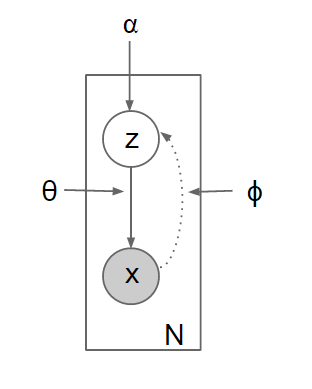
\includegraphics[width=1.2in]{images/model.png}
  \caption[]
   {Graphical representation of proposed model. $\alpha$ encodes the set of parameters for prior on $\mathbf{z}$, $\theta$ encodes the parameters for the generative model $p(\mathbf{x}|\mathbf{z})$, $\phi$ are the parameters for approximate posterior $p(\mathbf{z}|\mathbf{x})$}
  \label{fig:model}
\end{figure}

\subsection{Learning Factors of Variation with Known Block Structure}
We assume that the structure (size) of each block is known and this makes it easier to define the corresponding block diagonal covariance matrix. Such covariance matrix can be directly applied to the prior distribution $p(\mathbf{z})$ to guide the learning procedure. In addition, we could also easily parameterize the variational posterior distribution $q_{\phi}(\mathbf{z}|\mathbf{x})$ with Gaussian distribution with block diagonal covariance matrix, which will be discussed later.

The probabilistic graphical model is shown in Figure~\ref{fig:model}.
The generative process of $p_{\theta}(\mathbf{x}|\mathbf{z})$ is governed by Bernoulli or Gaussian MLP(Multilayer Perceptron), depends on the type of input data. We use $\theta$ to denote all the parameters of this MLP which include weight matrices and bias vectors. In particular, we assume $\mathbf{x}$ is generated from Gaussian distribution with mean $\mathbf{\eta}$ and diagonal covariance $\sigma^2\mathbf{I}$, where $\mathbf{\eta}$ and $\mathbf{\sigma}$ is generated from $\mathbf{z}$ via nonlinear transformation such that $\mathbf{\eta} = \mathbf{W}_2^\top\mathbf{h}_1 + \mathbf{b}_2$ and $\log \mathbf{\sigma}^2 = \mathbf{W}_3^\top\mathbf{h}_1 + \mathbf{b}_3$, and $\mathbf{h}_1 = \mbox{tanh}(\mathbf{W}_1^\top\mathbf{z} + \mathbf{b}_1)$. We define $\theta=(\mathbf{W}_1, \mathbf{W}_2,\mathbf{W}_3, \mathbf{b}_1, \mathbf{b}_2,\mathbf{b}_3)$.

The key component of our model is the prior distribution on $p(\mathbf{z})$. We assume $p(\mathbf{z})$ follows Gaussian distribution: $p(z)\sim N(\mu, \mathbf{\Lambda})$. In order to make $\mathbf{z}$ has disentangling effects, we enforce that the covariance matrix $\mathbf{\Lambda}$ has block diagonal structure. Since we know the number of blocks as well as the size of each block, we can explicitly define the structure of $\mathbf{\Lambda}$ as follows:
\begin{equation*}
\mathbf{\Lambda} = \begin{bmatrix}
\mathbf{\Lambda}_1 & 0 & 0 \\
0 & \ddots & 0  \\
0 & 0 & \mathbf{\Lambda}_{L}
\end{bmatrix} \\
\end{equation*}
Here $\mathbf{\Lambda}_1,...\mathbf{\Lambda}_L$ is the covariance matrix for each block and each size is known. Finally, we put the Normal-Wishart prior on each $\mathbf{\Lambda}_i$ such that $\mathbf{\mathbf{\Lambda}}_{i} \sim \mathcal{W}(\mathbf{\Lambda}_{i}; \mathcal{M}_{i}, \nu_{i})$. We denote $\vartheta=(\mathcal{M}_{1}, \nu_{1},...,\mathcal{M}_{L}, \nu_{L})$

The posterior distribution $p_{\theta}(\mathbf{z}|\mathbf{x})$, unfortunately, is intractable. Thus, we use variational distribution $q_{\phi}(\mathbf{z}|\mathbf{x})$ to approximate $p_{\theta}(\mathbf{z}|\mathbf{x})$.
In this work, we assume $q_{\phi}(\mathbf{z}|\mathbf{x})$ also follows Gaussian distribution with mean $\mu'$ and covariance $\mathbf{\Lambda}'$. The definition of $\mu'$ and $\mathbf{\Lambda}'$ is similar to the definition of $\mu$, $\mathbf{\Lambda}$, both of which follow the MLP. We also enforce that $\mathbf{\Lambda}'$ has block diagonal structure, and this assumption makes the generative process different from the one used in~\cite{kingma2013auto}. In particular for each $i$, we have $\mathbf{\Lambda}_i=\mathbf{A}_i\mathbf{A}_i^{\top}$, where matrix $\mathbf{A}_i^{\top}$ is generated via nonlinear transformation of $\mathbf{x}$ such that $\mathbf{A}_i=\exp(\mathbf{W}_{5,i}^{\top}\mathbf{h}_2+\mathbf{b}_{5,i})$ for $i=1,...,L$, and $\mathbf{h}_2=tahn(\mathbf{W}_4^{\top}\mathbf{x}+\mathbf{b}_4)$. In experimental section, we also tested the model with the covariance matrix has diagonal form instead of block diagonal. We denote $\phi=(\mathbf{W}_4, \mathbf{b}_4, \{\mathbf{W}_{5,i}\}_{i=1}^{L}, \{\mathbf{b}_{5,i}\}_{i=1}^{L})$.


\subsubsection{Variational Inference}
By following the standard procedure of variational inference, we can rewrite the log-probability of observation as
\[
\log P(\mathbf{x}) = D_{KL}(q_{\phi}(\mathbf{z}|\mathbf{x}) || p_{\theta}(\mathbf{z}|\mathbf{x})) + E_{q_{\phi}(\mathbf{z}|\mathbf{x})}[\log \frac{p_{\vartheta, \theta}(\mathbf{x},\mathbf{z})}{q_{\phi}(\mathbf{z}|\mathbf{x})}]
\]
The second term provides a variational likelihood
\[
\mathcal{L} = E_{q_{\phi}(\mathbf{z}|\mathbf{x})} \log p_{\theta}(\mathbf{x}|\mathbf{z}) - D_{KL}[q_{\phi}(\mathbf{z}|\mathbf{x})||p_{\vartheta}(\mathbf{z})] := \mathcal{L}_1 + \mathcal{L}_2
\]
We can learn the model parameters by maximizing $\mathcal{L}$ using stochastic gradient descent(SGD). Gradient of $\mathcal{L}_1$ w.r.t. parameters $\theta, \phi$ can be optimized using back-propagation algorithm by following the auto-encoding variable bayes procedure~\cite{kingma2013auto}. For the KL divergence term, we can also get the closed form formulation as below
\begin{align}
\notag \mathcal{L}_2 &:= \int_{(\mu, \mathbf{\Lambda})\sim NW(\mathbf{m}, \beta, \mathcal{M}, \nu)} KL(\mathcal{N}(\eta, \mathbf{\Sigma})||\mathcal{N}(\mu, \mathbf{\Lambda}^{-1})) \ d\mu d\mathbf{\Lambda} \\
\notag				& = -\frac{1}{2}\log|\mathbf{\Sigma}| - \frac{1}{2}[\log |\mathcal{M}| + \sum_{i=1}^{d}\psi(\frac{\nu-d+i}{2})] + \frac{\nu}{2}[\mbox{tr}(\mathcal{M}\mathbf{\Sigma})] + \frac{1}{2} [\frac{d}{\beta} + \nu \mbox{tr}(\mathcal{M}(\mbox{m}-\eta)(\mbox{m}-\eta)^{\top})]
\end{align}
where $\psi(\cdot)$ is the digamma function, and $\mathbf{m}, \beta$ are the prior parameters for $\mu$. Since the KL divergence term has analytic formulation, we can optimize the related parameters using SGD.


\begin{figure}[hb]
  \centering
  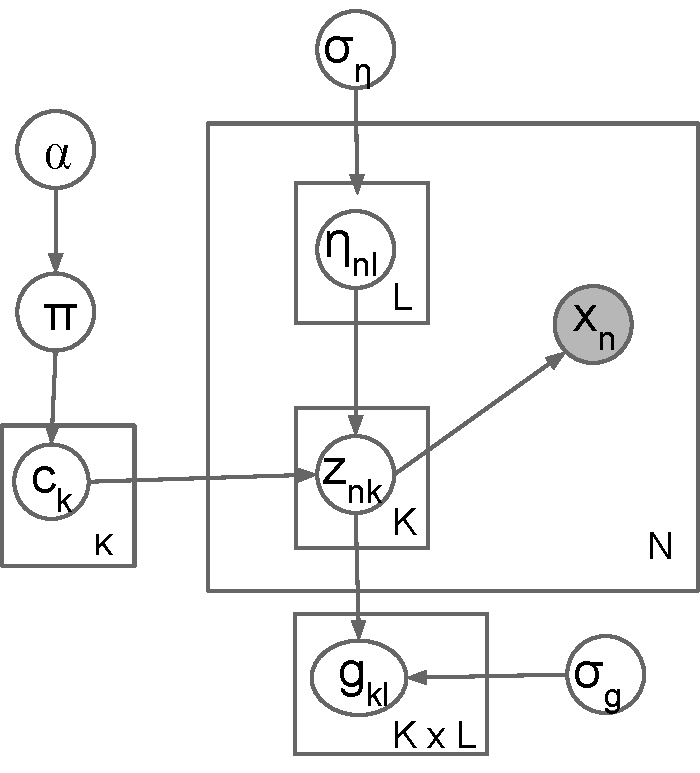
\includegraphics[width=1.8in]{images/blockmodel.pdf}
  \caption[]
   {Graphical representation of our proposed block diagonal prior model. $\alpha, \sigma_d, \sigma_g, \sigma_{\eta}$ are the hyperparameters. $\{c_k\}, \{g_{kl}\}, \{\eta_{nl}\}$ are the parameters of the prior model. $\{\mathbf{z_i}\}$ is the latent representation, and $\{\mathbf{x}_i\}$ are our observations. The difference between this model and our previous model is that we add additional generative process on top of $z$. The generative process of $p(x|z)$ and its corresponding posterior $q(z|x)$ remains the same, which are parameterized by $\theta, \psi$ respectively. }
  \label{fig:blockprior}
\end{figure}

\subsection{Learning Factors of Variation with Unknown Block Structure}

So far, we assume the size of each block is known. However, this assumption can be relaxed by putting variable clustering prior~\cite{palla2012nonparametric} on $p(\mathbf{z})\in R^K$. This prior is acted as another generative process which models the correlation within the cluster and assign the cluster membership to each dimension of latent representation. After incorporation of this prior, the new probabilistic model is depicted in Figure~\ref{fig:blockprior}, and the corresponding generative process is shown as below:

\begin{enumerate}[noitemsep]
\item Draw $\pi\sim \text{Dir}(\alpha)$
\item For each latent dimension $k$ from $1$ to $K$
    \begin{enumerate}[noitemsep]
    \item Draw dimension membership $c_k\sim \text{multinomial}(\pi)$
    \end{enumerate}
\item For each dimension $k=1...K, ~~l=1...L$
    \begin{enumerate}[noitemsep]
    \item Draw factor loading variable $g_{kl}\sim N(0, \sigma_g^2)$
    \end{enumerate}
\item For each sample $n=1...N$
    \begin{enumerate}[noitemsep]
        \item For each block/cluster $l=1...L$
        \begin{enumerate}
            \item Draw latent factor $\eta_{nl}\sim N(0, \sigma_{\eta})$
        \end{enumerate}
        \item For each dimension $k=1...K$
        \begin{enumerate}
            \item Draw latent representation $z_{nk}\sim N(g_{kc_k}\eta_{nc_k}, \sigma_k^2)$
        \end{enumerate}
        \item Draw each observation $\mathbf{x}_i \sim f_{\theta}(\mathbf{z}_i)$
    \end{enumerate}
\end{enumerate}

Here, $\alpha, \sigma_g, \sigma_k, \sigma_{\eta}$ are hyperparameters that we can fix beforehand\footnote{Of course, we could also learn these parameters. But in this paper, we treat them as hyperparameters and select the optimal ones using cross validation}. $\{\eta_{nl}\}$ is the local parameters that depends on $z_n$ while $\{g_{kc_k}\}$ are the global parameters that control the dimension membership. Based on this variable clustering prior model, the covariance of $\text{cov}(z_{nk}, z_{nk'}|\{g_{kl}\}, \{c_k\})$ as below
\[ \text{cov}(z_{nk}, z_{nk'}|\{g_{kl}\}, \{c_k\}) = \left\{
  \begin{array}{l l}
    \sigma_{\eta}^2g_{kc_k}g_{k'c_{k'}}+\sigma_d^2\delta_{kk'} & \quad \text{if $c_k=c_{k'}$}\\
    0 & \quad \text{otherwise}
  \end{array} \right.\]
This explicitly defines the block diagonal covariance structure, and enables the model to automatically learn the structure (size) of each block.  Besides the change of prior on $p(\mathbf{z})$, remaining stays the same. As before, we model $p_{\theta}(\mathbf{x}|\mathbf{z})$ using Gaussian distribution whose parameters are generated by MLP, and the variational distribution $q_{\phi}(\mathbf{z}|\mathbf{x})$ is also modeled by Gaussian distribution but with diagonal covariance matrix.

\subsubsection{Inference}
The learning for current model is more complicated than previous ones, which requires the sampling steps for parameters of prior model. We use the gibbs sampler to compute the expected values of $\mathbf{G}, \mathbf{C}$. After we compute those values, the conditional distribution $p(\mathbf{z}|\mathbf{G},\mathbf{C})$ can be obtained as the closed form formulation, which is made as the input to KL divergence term in the variational likelihood. The learning for the remaining part remains the same. The overall learning procedure is shown in Algorithm~\ref{alg:model}.

\paragraph{Sampling $\mathbf{G}$} $p(g_{kl}|\mathbf{C},\mathbf{G},\mathbf{\eta}, \mathbf{Z},\sigma_g)\sim \mathcal{N}(\mu_{g_{kl}}^*, \Lambda_{g_{kl}}^*)$, where
\[ \mu_{g_{kl}}^*, \Lambda_{g_{kl}}^* =
  \begin{cases}
     \mu_g, \sigma_g^{-2}      & \text{if} ~~c_{kl} = 0\\
    \left(\frac{\mu_g}{\sigma_g^2}+\frac{1}{\sigma_d^2}\sum_{n=1}^{N}\eta_{nl}z_{nk}\right)\Lambda_{g_{kl}}^{-1}, \frac{1}{\sigma_d^2}\left(\frac{\sigma_d^2}{\sigma_g^2}+\sum_{n=1}^{N}\eta_{kl}^2\right)  & \text{if}~~ c_{kl} = 1\\
  \end{cases}
\]
\paragraph{Sampling $\mathbf{\eta}$} $p(\eta_{nl}|\mathbf{C},\mathbf{G},\sigma_{\eta})\sim \mathcal{N}(\mu_{\eta_l}^*, \Lambda_{\eta_{l}}^*)$, where
\[
\mu_{\eta_l}^*, \Lambda_{\eta_{l}}^*={\Lambda_{\eta_l}^*}^{-1}\left(\frac{\mu_\eta}{\sigma_{\eta}^2}+\frac{\sum_{k=1}^{K}g_{kl}c_{kl}z_{nk}}{\sigma_d^2}\right),
\frac{1}{\sigma_{\eta}^2}+\frac{\sum_{k=1}^{K}g_{kl}^2c_{kl}^2}{\sigma_d^2}
\]
\paragraph{Sampling $\mathbf{C}$}
\textcolor{blue}{TODO: \@Dong  pls add here}

\begin{algorithm}[t]
\caption{Learning procedure for our model with unknown block structure}\label{alg}
\begin{algorithmic}[1]
\STATE initialize $\sigma_k, \sigma_g, \sigma_{\eta}$
\STATE initialize $\pi, \{c_d\}, \{g_{dk}\}$ by drawing from Gaussian distributions.
\FOR{ epoch=1...Max\_{epoch} (one pass over the whole training set)}
\FOR {each mini-batch $D$}
\STATE Run forward propagation on $D$ and compute $Z$.
\STATE Run gibbs sampler to compute $p(\eta_{nl}|\{z_{nk}\}, \{c_k\}, \{g_{kl}\}), ~~p(\{g_{kl}\}|\{z_{nk}\},\{c_k\}, \{\eta_{nl}\})$\\
$p(\{c_k\}|\{z_{nk}\},\{g_{kl}\}, \theta, \{\eta_{nl}\}), ~~p(\pi|\alpha,\{c_k\})$, and update using averaged samples.
\STATE Compute $p(z|\{g_{kl}^*\},\{c_k^*\})$
\STATE Learn the model parameters $\theta$ and $\phi$ using SGD (same as before).
\ENDFOR
\ENDFOR
\end{algorithmic}
\label{alg:model}
\end{algorithm}














\iffalse

\paragraph{Generative model for $p(\mathbf{x}|\mathbf{z};\theta)$}  We assume $\theta=(\mathbf{W}_4^T, \mathbf{W}_5^T,\mathbf{W}_6^T, \mathbf{b}_4, \mathbf{b}_5,\mathbf{b}_6)$

\begin{align}
& p(\mathbf{x}|\mathbf{z}) = \mathcal{N}(\eta, \sigma^2\mathbf{I}) \\
& \eta = \mathbf{W}_5^T\mathbf{h}_2 + \mathbf{b}_5 \\
& \log \sigma^2 = \mathbf{W}_6^T\mathbf{h}_2 + \mathbf{b}_6 \\
& \mathbf{h}_2 = \mbox{tanh}(\mathbf{W}_4^T\mathbf{z} + \mathbf{b}_4)
\end{align}


\paragraph{Prior model for $p(\mathbf{z})$}
We introduce a block diagonal regularizer by modeling the prior distribution of $\mathbf{z}$ as block diagonal Gaussian. We assume $\alpha=(\mathcal{M}_{1}, \nu_{1},...,\mathcal{M}_{k},\nu_{k})$
\begin{align}
& p(\mathbf{z}| \mathbf{\Lambda}) = \mathcal{N}(\mathbf{m},\mathbf{\Lambda)}, \mbox{where} \nonumber\\
& \mathbf{\Lambda} = \begin{bmatrix}
\mathbf{\Lambda}_1 & 0 & 0 \\
0 & \ddots & 0  \\
0 & 0 & \mathbf{\Lambda}_{K}
\end{bmatrix} \\
& \mathbf{\Lambda}_{i} \sim \mathcal{W}(\mathbf{\Lambda}_{i}; \mathcal{M}_{i}, \nu_{i})\\
& p_{\alpha}(\mathbf{z}) = \prod_{k=1}^{K}  \int N(\mathbf{m}_k, \mathbf{\Lambda}_k) \mathcal{W}(\mathbf{\Lambda}_{k}; \mathcal{M}_{k}, \nu_{k}) d\mathbf{\Lambda}
\end{align}

\paragraph{Posterior model for $q(\mathbf{z}|\mathbf{x};\phi)$}
The approximate posterior model $q(\mathbf{z}|\mathbf{x};\phi)$ is
\begin{align}
& q_{\phi}(\mathbf{z}|\mathbf{x})=N(\mu', \mathbf{\Lambda}) \\
& \mu' = \mathbf{W}_2^T h_1 + \mathbf{b}_2 \\
&\mathbf{\Lambda} = \begin{bmatrix}
\mathbf{\Lambda}_1 & 0 & 0 \\
0 & \ddots & 0  \\
0 & 0 & \mathbf{\Lambda}_{K}
\end{bmatrix} \\
& \mathbf{\Lambda_k} = \mathbf{A}_k\mathbf{A}_k^{\top}\\
& \mathbf{A}_k= \exp(\mathbf{W}_{3k}^{\top}h_1 + \mathbf{b}_{3k})\\
%& \sigma(\mathbf{x}, \mathbf{W}_1, \mathbf{W}_3) = A(\mathbf{x},\mathbf{W}_1,\mathbf{W}_3)\cdot A^T(\mathbf{x},\mathbf{W}_1,\mathbf{W}_3)\\
& h_1 = \mbox{tahn}(\mathbf{W}_1^T\mathbf{x} + \mathbf{b}_1)
\end{align}


\subsubsection{Variational Inference}
By following the standard procedure of variational inference, we can rewrite log-probability of observation as
\begin{align}
\log P(\mathbf{x}) = D_{KL}(q_{\phi}(\mathbf{z}|\mathbf{x}) || p_{\theta}(\mathbf{z}|\mathbf{x})) + E_{q_{\phi}(\mathbf{z}|\mathbf{x})}[\log \frac{p_{\alpha, \theta}(\mathbf{x},\mathbf{z})}{q_{\phi}(\mathbf{z}|\mathbf{x})}]
\end{align}
The second term provides a variational likelihood
\begin{align}
\mathcal{L} = E_{q_{\phi}(\mathbf{z}|\mathbf{x})} \log p_{\theta}(\mathbf{x}|\mathbf{z}) - D_{KL}[q_{\phi}(\mathbf{z}|\mathbf{x})||p_{\alpha}(\mathbf{z})] := \mathcal{L}_1 + \mathcal{L}_2
\end{align}

We can learn the model by maximizing $\mathcal{L}$ using SGD. Gradient of $\mathcal{L}_1$ w.r.t. parameters $\theta, \phi$ can be calculated using back-propagation algorithm, by following the auto-encoding variable bayes procedure. For the KL divergence term, we could also get the closed form formulation, which can be optimized SGD as well.


\begin{figure}
        \centering
        \begin{subfigure}[b]{0.3\textwidth}
                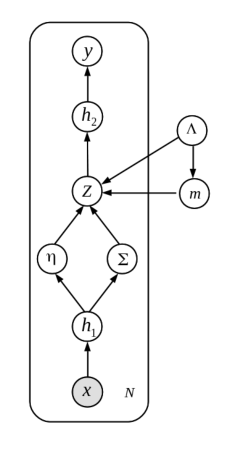
\includegraphics[width=\textwidth]{model2}
                \label{fig:gull}
        \end{subfigure}%
        ~ %add desired spacing between images, e. g. ~, \quad, \qquad, \hfill etc.
          %(or a blank line to force the subfigure onto a new line)
        \begin{subfigure}[b]{0.37\textwidth}
                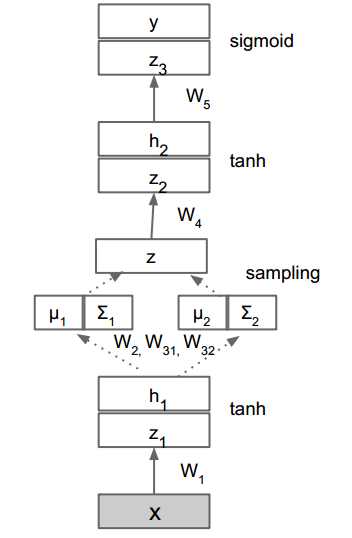
\includegraphics[width=\textwidth]{model1}
                \label{fig:tiger}
        \end{subfigure}
        ~ %add desired spacing between images, e. g. ~, \quad, \qquad, \hfill etc.
        \caption{(a) Graph representation of proposed model. The only observation here is the input $x$. $\Lambda, m$ are modeled by normal-wishart prior. (b) The detailed flow of transforming $x$ to reconstruction $y$. The nonlinear transformation function are denoted on the right hand side}
\end{figure}


\subsubsection{Optimizing likelihood term}
Figure 2-(b) shows the detailed auto-encoding procedure for likelihood term. It shows the case where we have two blocks. Below is the list of transformations denoted by this figure.
\begin{align}
\mathbf{h}_1&=tanh(\mathbf{W}_1^{\top}\mathbf{x})\\
\mathbf{\mu}_1&=\mathbf{W}_{21}^{\top}\mathbf{h}_1\\
\mathbf{\mu}_2&=\mathbf{W}_{22}^{\top}\mathbf{h}_1\\
\log \mathbf{A}_1 &= \mathbf{W}_{31}^{\top}\mathbf{h}_1\\
\log \mathbf{A}_2 &= \mathbf{W}_{32}^{\top}\mathbf{h}_1\\
\mathbf{\mu} &= [\mathbf{\mu}_1, \mathbf{\mu}_2] \\
\mathbf{A} &= [\mathbf{A}_1, 0; 0, \mathbf{A}_2] \\
\mathbf{z}^{(l)}&=\mathbf{\mu} + \mathbf{A} \mathbf{\epsilon}^{(l)}, ~~~\mathbf{\epsilon}^{(l)} \sim \mathcal{N}(0, \mathbf{I})\\
\mathbf{h}_2^{(l)} &= tanh(\mathbf{W}_4^{\top}\mathbf{z}^{(l)})\\
\mathbf{y}^{(l)} &= \sigma(\mathbf{W}_5^{\top}\mathbf{h}_2^{(l)})
\end{align}


If our input data is the binary images (i.e MNIST), then the likelihod  thus the likelihood term for specific sample $x$ can be written as (if input data is continuous images, we use $l_2$ reconstruction loss) :
\[
\mathcal{L}^{(l)} = \sum_{d=1}^{D_0}x_d\log y_d^{(l)}+(1-x_d)\log(1-y_d^{(l)})
\]
During the learning procedure, we need to generate multiple latent representations by combining different random noise with the given data $x$. This is the reason why we use superscript $(l)$ to denote the specific version of latent representation for input $x$.

Given this likelihood term, the gradient w.r.t each hidden variable can be written as:
\begin{align}
\frac{\partial \mathcal{L}^{(l)}}{\partial \mathbf{z}_3} &= \mathbf{x}-\mathbf{y}^{(l)} \\
\frac{\partial \mathcal{L}^{(l)}}{\partial \mathbf{z}_2} &= (\mathbf{W}_5 \frac{\partial \mathcal{L}^{(l)}}{\partial \mathbf{z}_3}) \odot (1-\mathbf{h}^2)\\
\frac{\partial \mathcal{L}^{(l)}}{\partial \mathbf{z}} &= \mathbf{W}_4 \frac{\partial \mathcal{L}^{(l)}}{\partial \mathbf{z}_2}\\
\frac{\partial \mathcal{L}^{(l)}}{\partial \mathbf{A}} &= \frac{\partial \mathcal{L}^{(l)}}{\partial \mathbf{z}} {\mathbf{\epsilon}^{(l)}}^{\top}, ~~~  \mathbf{\epsilon}^{(l)} \sim \mathcal{N}(0, \mathbf{I}) \\
\frac{\partial \mathcal{L}^{(l)}}{\partial \mathbf{z}_1}&=(W_2\frac{\partial \mathcal{L}^{(l)}}{\partial \mathbf{\mu}}+W_3(\frac{\partial \mathcal{L}^{(l)}}{\partial \mathbf{A}})\odot \mathbf{A}) \odot (1-{\mathbf{h}_1}^2)\\
\frac{\partial L^{1}}{\partial \mu}&= \frac{\partial L^{(1)}}{\partial z}
\end{align}

Finally, the gradient for each parameter is:
\begin{align}
\frac{\partial \mathcal{L}^{(l)}}{\partial \mathbf{W}_5}&=\mathbf{h}_2^{(l)} (\frac{\partial \mathcal{L}^{(l)}}{\partial \mathbf{z}_3})^{\top} \\
\frac{\partial \mathcal{L}^{(l)}}{\partial \mathbf{W}_4} &= \mathbf{z}(\frac{\partial \mathcal{L}^{(l)}}{\partial \mathbf{z}_2})^{\top}\\
\frac{\partial \mathcal{L}^{(l)}}{\partial \mathbf{W}_3} &= \mathbf{h}_1 (\frac{\partial \mathcal{L}^{(l)}}{\partial \mathbf{A}}\odot \mathbf{A} )^{\top}\\
\frac{\partial \mathcal{L}^{(l)}}{\partial \mathbf{W}_2} &= \mathbf{h}_1 (\frac{\partial \mathcal{L}^{(l)}}{\partial \mathbf{\mu}})^{\top}\\
\frac{\partial \mathcal{L}^{(l)}}{\partial \mathbf{W}_1} &= \mathbf{x}(\frac{\partial \mathcal{L}^{(l)}}{\partial \mathbf{z}_1})^{\top}
\end{align}


\subsubsection{Optimizing KL divergence term}
We put the normal-wishart prior on the parameters of the normal distributions. This is equivalent to integrating out all possible normal distribution parameters. The derivation of KL divergence term is shown as below:

\begin{align}
\notag \mathcal{L}_{KL} &:= \int_{(\mu, \Lambda)\sim NW(\mathbf{m}, \beta, W, \nu)} KL(\mathcal{N}(\eta, \Sigma)||\mathcal{N}(\mu, \Lambda^{-1})) \ d\mu d\Lambda \\
\notag				& :=  \int_{(\mu, \Lambda)\sim NW(\mathbf{m}, \beta, W, \nu)}  \frac{1}{2}[-\log(|\Lambda|) - \log(|\Sigma|) -d + \mbox{tr}(\Lambda\Sigma) + (\mu-\eta)^T\Lambda(\mu-\eta)]\ d\mu d\Lambda \\
\notag				& = -\frac{1}{2}\log|\Sigma| - \frac{1}{2}E_{\mu, \Lambda}[\log |\Lambda|] + \frac{1}{2}E_{\mu, \Lambda} [\mbox{tr}(\Lambda\Sigma)] + \frac{1}{2} E_{\mu, \Lambda}[(\eta-\mu)^T\Lambda(\eta-\mu)]\\
\notag				& = -\frac{1}{2}\log|\Sigma| - \frac{1}{2}[\log |W| + \sum_{i=1}^{d}\psi(\frac{\nu-d+i}{2})] + \frac{\nu}{2}[\mbox{tr}(W\Sigma)] + \frac{1}{2} [\frac{d}{\beta} + \nu \mbox{tr}(W(\mbox{m}-\eta)(\mbox{m}-\eta)^T)]
\end{align}

where $\psi(\cdot)$ is the digamma function. Discarding the terms irrelevant to $\eta, \Sigma$, we can obtain a simplified formulation of KL divergence part in objective function:
\begin{align}
\label{KLW} \mathcal{L}_2 := \frac{1}{2} \sum_{n=1}^{N} \log|\Sigma| - \mbox{tr}(\nu W \Sigma ) - (\mathbf{m}-\eta)^T \nu W (\mathbf{m}-\eta)
\end{align}





\subsection{Putting block diagonal prior on $p(\mathbf{z})$}

\begin{figure}[hb]
  \centering
  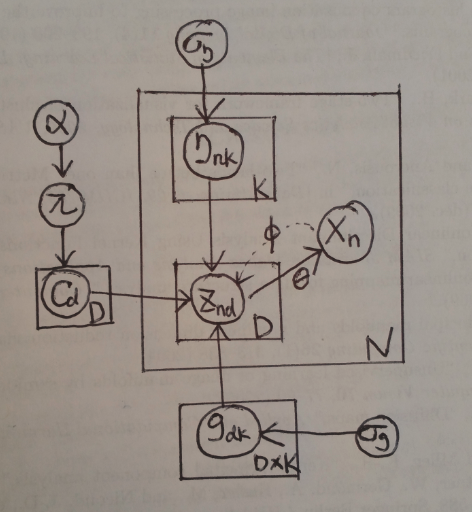
\includegraphics[width=2in]{blockmodel.png}
  \caption[]
   {Graphical representation of our proposed block diagonal prior model. $\alpha, \sigma_d, \sigma_g, \sigma_{\eta}$ are the hyperparameters. $\{c_d\}, \{g_{dk}\}, \{\eta_{nk}\}$ are the parameters of the prior model. $\{\mathbf{z_i}\}$ is the latent representation, and $\{\mathbf{x}_i\}$ are our observations. The difference between this model and our previous model is that we add additional generative process on top of $z$. The generative process of $p(x|z)$ and its corresponding posterior $q(z|x)$ remains the same, which are parameterized by $\theta, \psi$ respectively.}
\end{figure}


For now, we assume the number of blocks $K$, is known. But this can be easily generalized to the nonparametric case, by using Dirichlet process. The core idea of block prior is given in~\cite{palla2012nonparametric} and the draft by Ren and Emily Fox.

By incorporating the block diagonal prior, the generative process of our model is given below:

\begin{enumerate}[noitemsep]
\item Draw $\pi\sim Dir(\alpha)$
\item For each latent dimension $d$ from $1$ to $D$
\item $~~~~$Draw dimension membership $c_d\sim multinomial(\pi)$
\item For $d=1...D, ~~k=1...K$
\item $~~~~$Draw factor loading variable $g_{dk}\sim N(0, \sigma_g^2)$
\item For each sample $n=1...N$
\item $~~~~$For each block/cluster $k=1...K$
\item $~~~~~~~~$Draw latent factor $\eta_{nk}\sim N(0, \sigma_{\eta})$
\item $~~~~$For $d=1...D$
\item $~~~~~~~~$Draw latent representation $z_{nd}\sim N(g_{dc_d}\eta_{nc_d}, \sigma_d^2)$
\item $~~~~$Draw $x_i \sim f_{\theta}(z_i)$
\end{enumerate}

Based on this block diagonal prior model, we could get

\[ cov(z_{nd}, z_{nd'}|\{g_{dk}\}, \{c_d\}) = \left\{
  \begin{array}{l l}
    \sigma_{\eta}^2g_{dc_d}g_{d'c_{d'}}+\sigma_d^2\delta_{dd'} & \quad \text{if $c_d=c_{d'}$}\\
    0 & \quad \text{otherwise}
  \end{array} \right.\]

Please note that when we draw $x_i$ from $z_i$, we use MLP as before. Also, we model the posterior $p(z|x)$ as diagonal covariance matrix. (we could also use full covariance matrix). We treat $\sigma_d, \sigma_{\eta}, \sigma_g$ as hyperparameters, which we fix beforehand. (of course, we can also learn these parameters as well).

\section{Learning the model}
The learning procedure is in Algorithm 1. Basically, there are two large components in our model, one is our previous MLP model (similar to Max Welling's formulation), and the other one is the block diagonal prior we impose. For the latter one, we use gibbs sampling. The latent representation $\mathbf{Z}$ is the bridge between these two components. And we alternatively optimize these two components.


\begin{algorithm}[t]
\caption{Learning procedure for our model}\label{alg}
\begin{algorithmic}[1]
\STATE initialize $\sigma_d, \sigma_g, \sigma_{\eta}$
\STATE initialize $\pi, \{c_d\}, \{g_{dk}\}$ by drawing from corresponding distributions.
\FOR{iteration $\text{itr}=1...\text{Max_itr}$ (one pass over the whole training set)}
\FOR {each mini-batch $D$}
\STATE Run forward propagation on $D$ and compute $Z$.
\STATE Run gibbs sampler to compute $p(\eta_{nl}|\{z_{nk}\}, \{c_k\}, \{g_{kl}\}), ~~p(\{g_{kl}\}|\{z_{nk}\},\{c_k\}, \{\eta_{nl}\})$\\
$p(\{c_k\}|\{z_{nk}\},\{g_{kl}\}, \theta, \{\eta_{nl}\}), ~~p(\pi|\alpha,\{c_k\})$, and update using averaged samples.
\STATE Compute $p(z|\{g_{kl}\},\{c_k\},\sigma_k)$
\STATE Learn the model parameters $\theta$ and $\phi$ using backpropagation (as we did before).
\ENDFOR
\ENDFOR
\end{algorithmic}
\end{algorithm}

\fi


\section{Experiment}
We validate our approaches on several image datasets.  The evaluation are mainly based on qualitative and qualitative results. For the qualitative evaluation, we examine the quality of the samples generated from our models (fixing one block while sampling from another), we do data exploration of learned representations using clustering plots, and we also analyze the correlation matrix learned by our methods. In terms of quantitative results, we provide the classification accuracy for the prediction task using learned latent representations. Results and discussions are provided in later sections.

\subsection{Setup}
\paragraph{Data} We evaluate our methods on $3$ image datasets: MNIST dataset~\footnote{http://yann.lecun.com/exdb/mnist/}, Face dataset~\footnote{http://www.multipie.org/} and Norb dataset~\footnote{http://www.cs.nyu.edu/~ylclab/data/norb-v1.0/}. MNIST contains $50,000$ training and $10,000$ testing samples from 10 different digit classes, and each image mainly contains two factors of variation: digit class and writing style. The face dataset contains the human face images from $68$ identities with different lighting conditions and views, which in total provides $3$ different factors\footnote{We use only subset of the original dataset.}. The Norb dataset also contains 3 factors including category, orientation and brightness\footnote{In fact, the Norb dataset contains more than 3 factors such as category, subcategory.etc. But in this experiments, we manually merge some of the factors which gives us total 3 factors in the end}.

\paragraph{Details} For each dataset, we convert the image pixel values of each dimension into normal distribution with mean zero and unit variance. We evaluate the performance on several models which are the combinations of different prior and variational posterior distributions. The summary of the proposed models and baseline model are shown in Table~\ref{table:model}

The model A is the baseline from \cite{kingma2013auto}, which assumes $\mathcal{N}(0,1)$ prior on $p(\mathbf{z})$ and Gaussian distribution with diagonal covariance $\mathcal{N}(\mu, \sigma^2\mathbf{I})$ for variational posterior distribution $q_{\phi}(\mathbf{z}|\mathbf{x})$

The model B and C are the ones trained with known block structure (i.e the number of blocks, and the size of each block). We put Gaussian distribution with block diagonal covariance $\mathcal{N}(\mu, \Lambda)$ on $p(\mathbf{z})$, where we explicitly parameterize $\Lambda$ with $L$ sub-blocks whose size are known. The main difference between model B and model C is that we use different forms of covariance to parameterize the variational posterior distribution $q_{\phi}(\mathbf{z}|\mathbf{x})$. For model B, we use Gaussian distribution with diagonal covariance $\mathcal{N}(0,\sigma^2\mathbf{I})$. On the other hand, for model C, we parameterize it using block diagonal covariance, where each sub-block is generated from MLP.

The model D and E are the generalization of model B and C to the case that the block structure is unknown (but we know the number of blocks $K$). The only difference is that we use block diagonal covariance to parameterize the posterior distribution for model D, while we use full covariance for model E.

The model G and F further generalize the model D and E. We use Chinese restaurant process (CRP) to infer the number $K$ from the data, instead of explicitly defining it beforehand. 

The model $\text{B}^*$ and $\text{C}^*$ are the supervised versions of model B and C, respectively. We add the supervised loss on one block of latent representation $z$. 

Finally, the model H is one baseline that we don't assume any structure on the prior or variational posterior. 

\begin{table}
\centering
\begin{tabular}{|l|c|c|c|c|c|c|}
\hline
\backslashbox{Posterior}{Prior}  & Full & $\mathcal{N}(0,1)$ & BLK(NW) & BLK(Factor) & DP Prior & S-BLK(NW) \\
\hline
 Diagonal& & Model $A$ & Model B & Model D & Model G & Model $\text{B}^*$ \\
 \hline
 BLK &  & & Model C& && Model $\text{C}^*$ \\
 \hline
 Full & Model H& &&Model E& Model F & \\
% & all & all\\
\hline
\end{tabular}
\caption{The summary of the models evaluated in this paper}
\label{table:model}
\end{table}


\subsection{MNIST datset}
\paragraph{Learning with $4$ hidden units and $2$ blocks}
We assume the size of hidden units is $4$, and the input data has two factors of variation. For model B and C, we define the covariance matrix having two $2$ by $2$ sub-blocks on the diagonal. This enforces that the first two hidden units control one factor, and the remaining two control the second factor, but we don't define which factor controls digit class or writing style before learning the model. For model A, since we don't explicitly define the grouping structures of hidden units, we need to do greedy search to figure out the group of hidden units control each of the factors. On the other hand, model D can automatically discover the group of hidden units without defining the structure. This brings one significant benefit in the cases that some factors contain much more information than others, and we expect that model D is able to assign more hidden units to those complex factors and less to the simpler ones. We will demonstrate some interesting observations in later section.


\paragraph{Quality of samples from different models}
\begin{figure}
\centering
    \begin{subfigure}[b]{0.9\textwidth}
    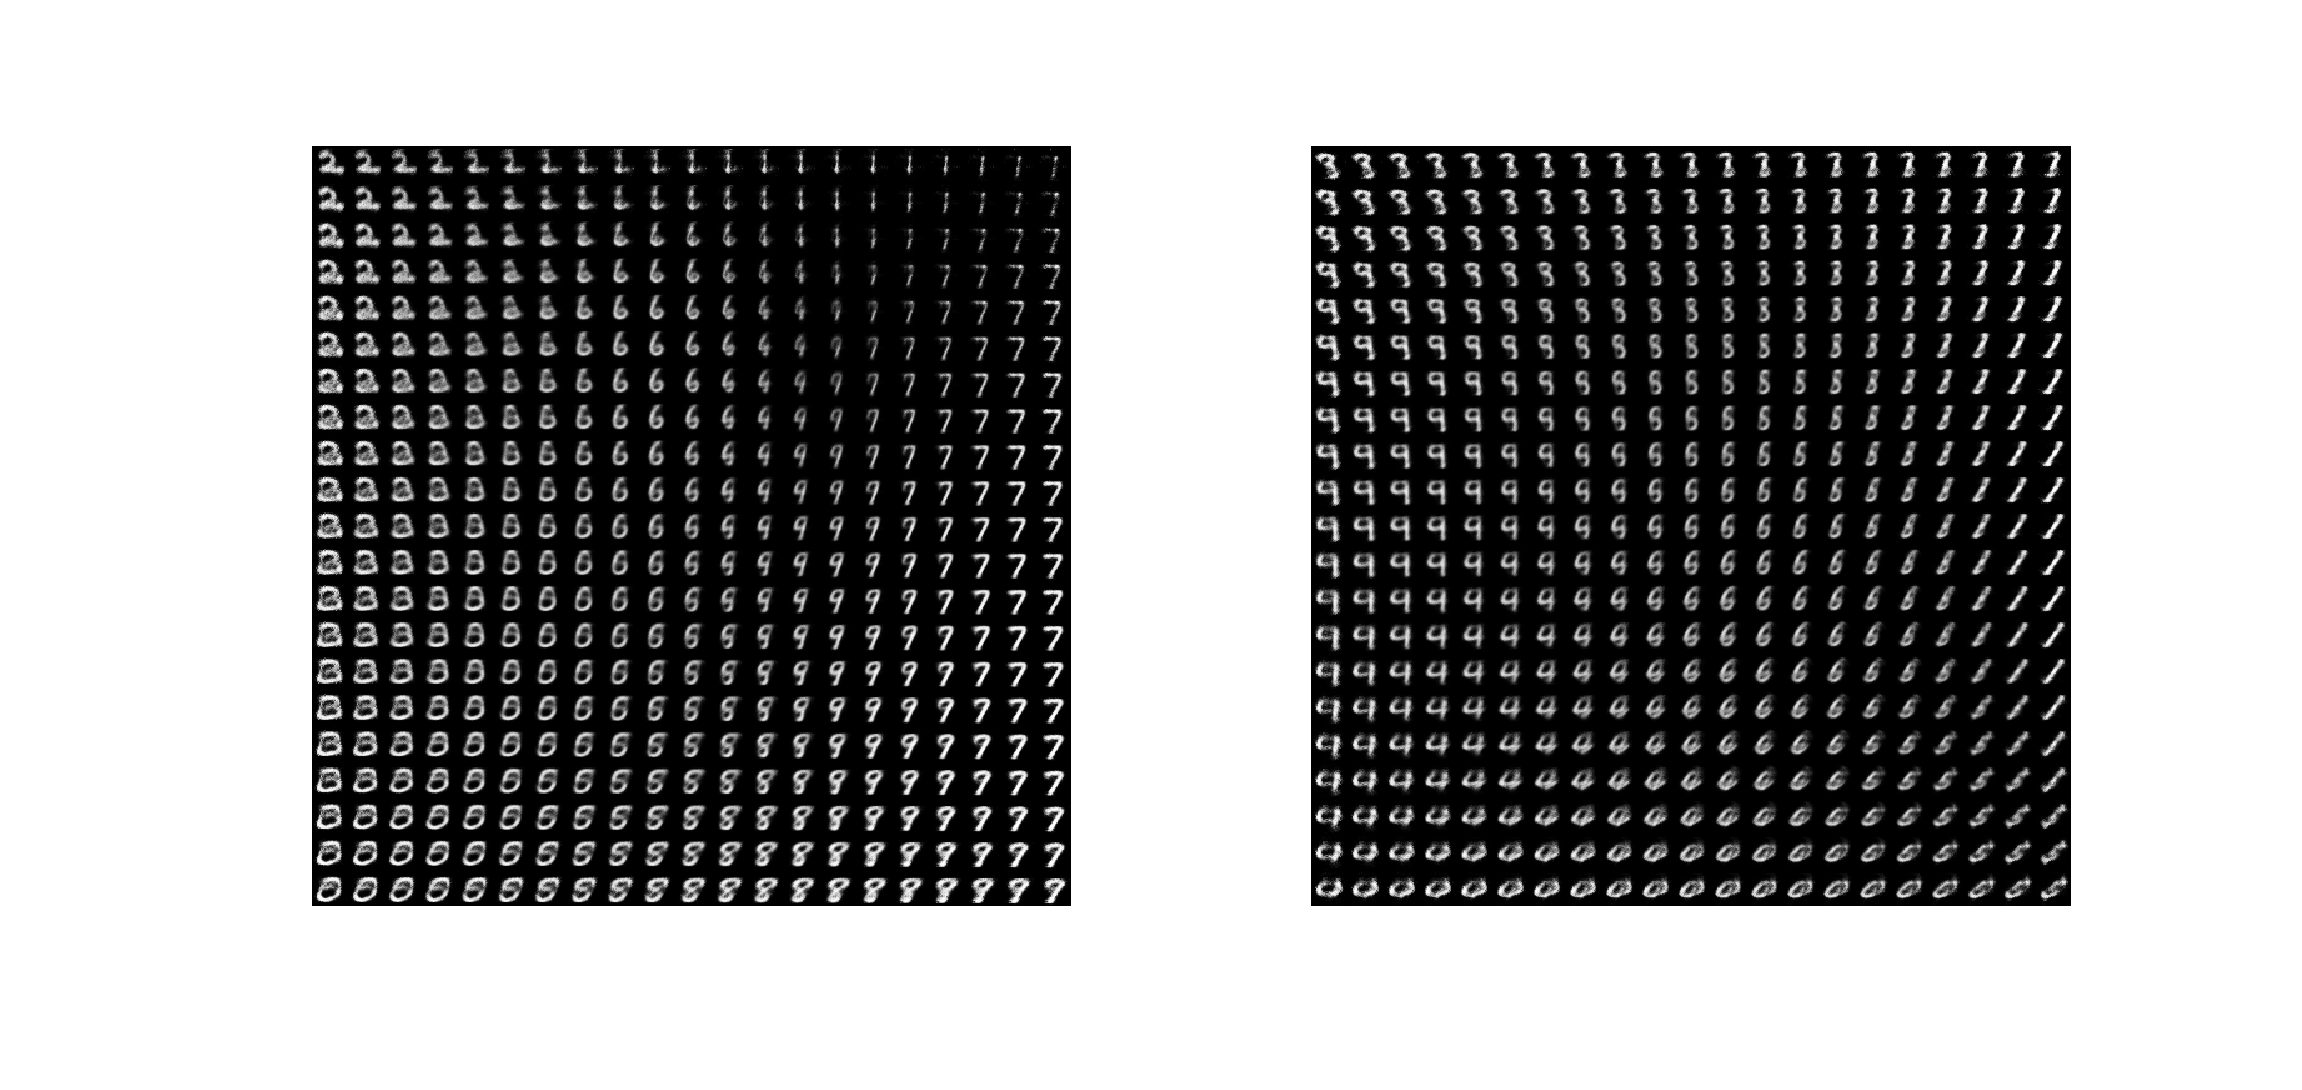
\includegraphics[width=\textwidth]{images/sampleWelling.eps}
    \vspace{-3\baselineskip}
    \caption{Model A}
    \label{fig:us-air}
    \end{subfigure}
	\begin{subfigure}[b]{0.9\textwidth}
    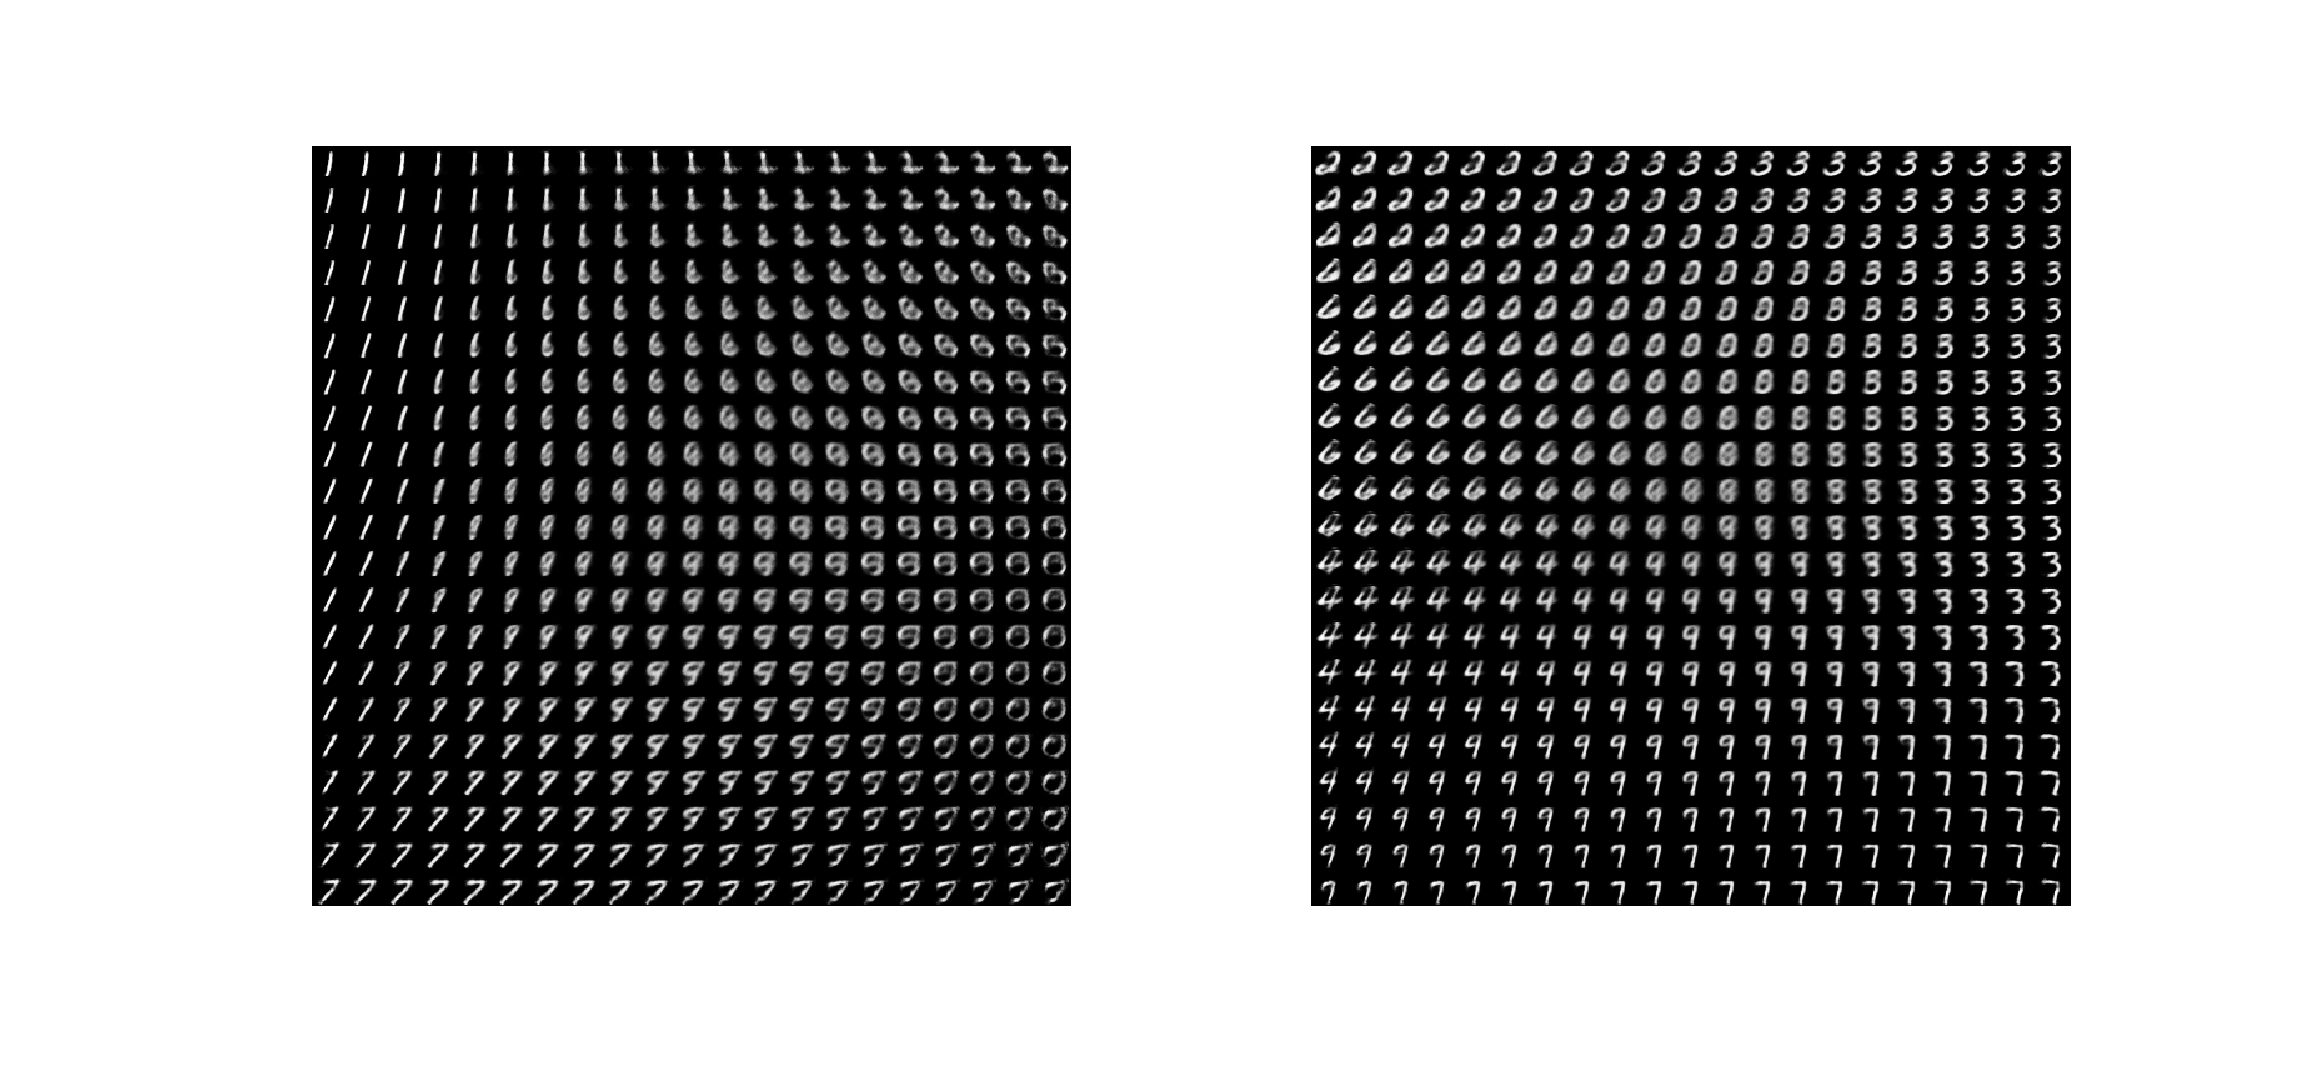
\includegraphics[width=\textwidth]{images/sampleNWdiag.eps}
    \vspace{-3\baselineskip}
    \caption{Model B}
    \label{fig:us-air}
    \end{subfigure}
    \begin{subfigure}[b]{0.9\textwidth}
    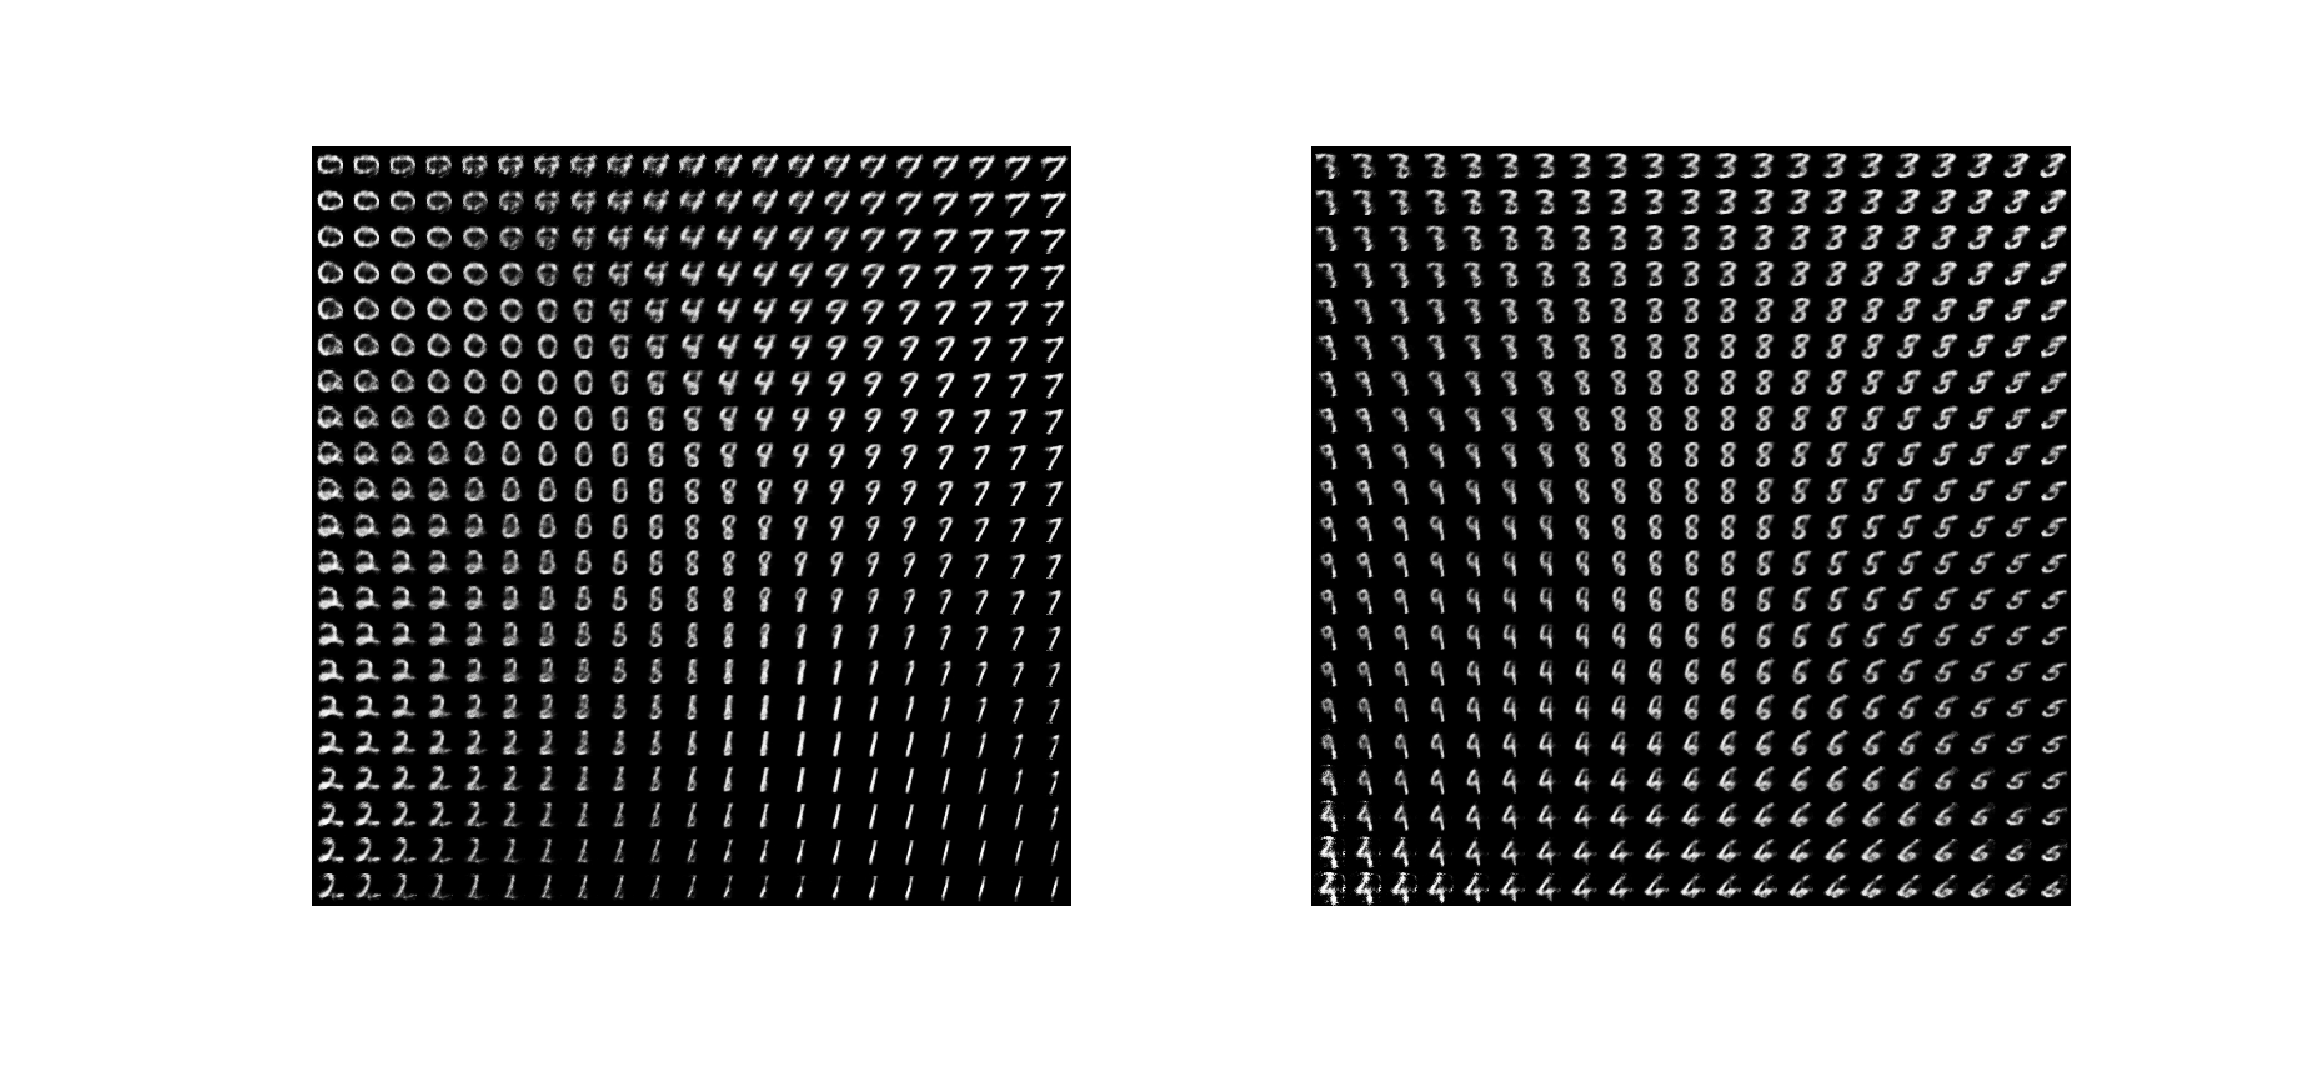
\includegraphics[width=\textwidth]{images/sampleNWblock.eps}
    \vspace{-3\baselineskip}
    \caption{Model C}
    \label{fig:us-air}
    \end{subfigure}
    \begin{subfigure}[b]{0.9\textwidth}
    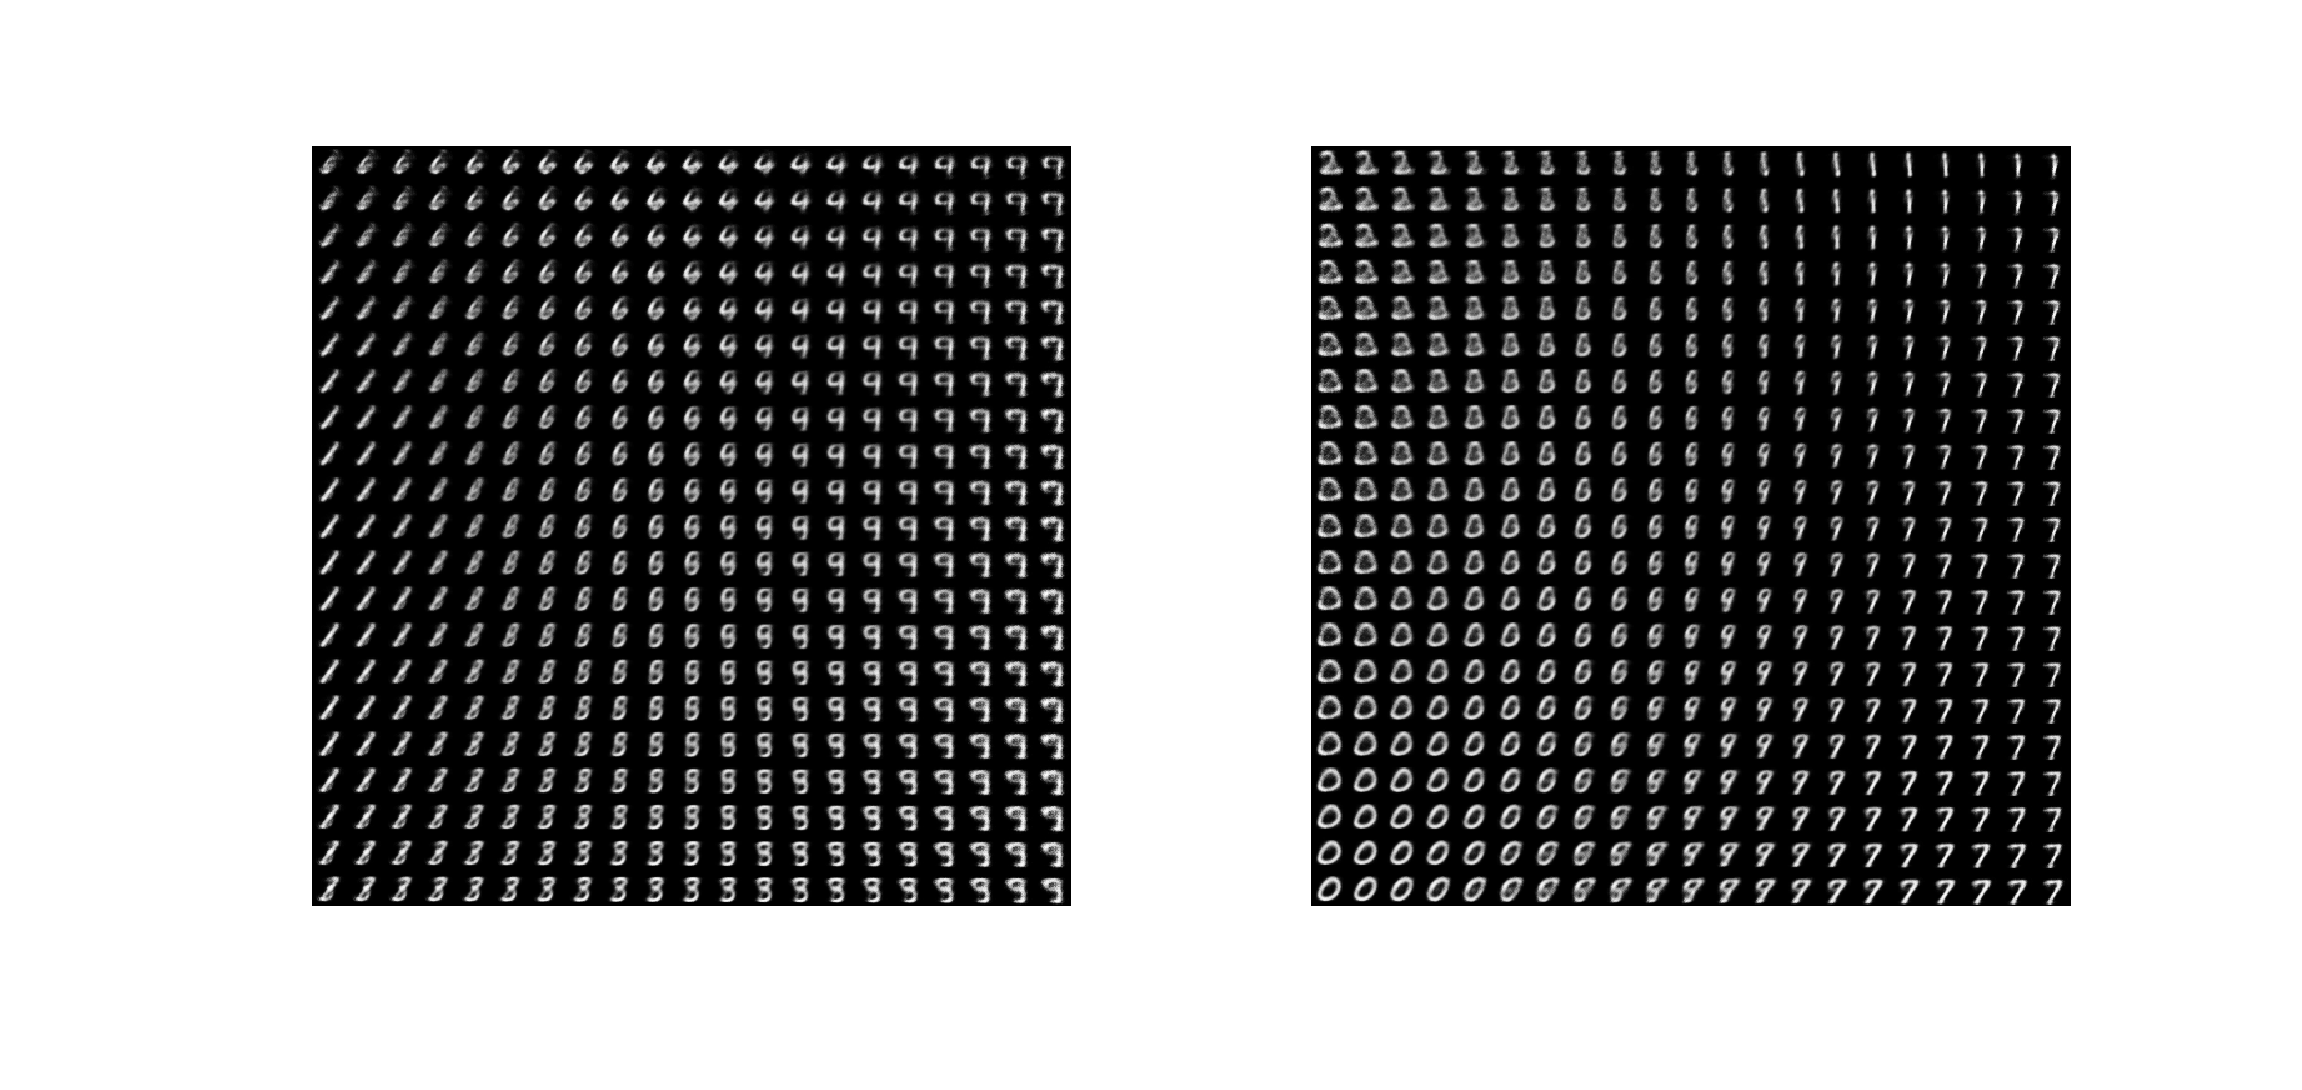
\includegraphics[width=\textwidth]{images/sampleAverage.eps}
    \vspace{-3\baselineskip}
    \caption{Model D}
    \label{fig:us-air}
    \end{subfigure}
    \caption{Generated samples from each model on MNIST dataset. The left figure shows the samples by fixing the first block (mean sample), and sample for the second block. Similar analogy applies to the right figure.}\label{fig:animals}
    \label{fig:MNISTsamples}
\end{figure}

Figure~\ref{fig:MNISTsamples} shows the generated samples from different models. The samples are generated by fixing one block and sample on another. By fixing we mean that we use the "mean" sample. In order to cover the sample space more broadly, we divide the space into grids and uniformly sample within that grid. The figure shows some interesting observations in terms of change of digit class and writing style. For model A, we could easily see that the digit class and writing style mixed together. The model B, although it's a bit better than model A, it's still hard to see the dominant factors for each block. However, for model C and D, the different is more distinguishable. The writing style factor dominates in the right figure of model C, and left figure of model D. And the remaining figures denote the change of digit classes. Please note that for this dataset, model D learns to assign two hidden units to one factor, and the other two for another factor.

\vspace{-0.1cm}
\paragraph{Predictive accuracy on the learned representations}
We also evaluate the predicative performance on the learned representation $\mathbf{z}$. For this purpose, we run the multinomial logistic regression on each block, and record the maximum accuracy. We expect that the factor encodes the digit class gives better prediction accuracy. Table~\ref{tab:regression} shows the classification results on MNIST dataset. The notation MNIST($4d_{\text{factor}}$) means that the classification accuracy is computed using one factor from the model that trained with $4$ hidden units, and MNIST($4d_{\text{all}}$) means that the result is computed using all the hidden units.

\begin{table*}[htb]
	\begin{center}
		\begin{small}
			\begin{sc}
				\begin{tabular}{lcc}
					\hline
					Data set & MNIST(4D\_factor) & MNIST(4D\_all)  \\
					\hline
					Model A& 53.9  & 74.6\\
					Model B &44.4 & 77.4\\
					Model C & 56.7 &80.5\\
					Model D & 48.2 & 71.6\\
					\hline
					% & all & all\\
				\end{tabular}
			\end{sc}
		\end{small}
        \vspace{0.2cm}
		\caption{Predictive performance on the hidden representation which encodes the digit class factor}
\vspace{-0.5cm}		
\label{tab:regression}
	\end{center}
\end{table*}

The difference between these models is not obvious. In general, the model with block diagonal prior and block diagonal variational posterior performs best. This is reasonable since we explicitly define the block structure which is equivalent to putting hard constraints. Although the model D does give least accuracy when we using all the hidden units, the performance on the digit factor is reasonablely good. The baseline model A gives the best accuracy when we only consider the digit factor. But please note that this factor is found by greedy search which provides the best accuracy, which might be unfair for comparisons with other models.

\subsection{Face dataset}
Face dataset contains $3$ factors. However, the image is more complicated than MNIST dataset, which means that each image contains more information. Thus, for this experiment, we increase the number of hidden units to $6$. Figure~\ref{fig:FacesamplesModel3} shows the generated samples from model C. We set the size of each factor having $2$ hidden units. From this figure, we can easily see that block 1 encodes identity, block 2 encodes brightness and block 3 encodes view factor.

More interesting experiments are for model D. Figure~\ref{fig:Facesamples} shows the generated samples from model D by sampling from one block while fixing others (with mean sample). From the figure, we can easily see that the block 1 controls the lighting condition, block 2 controls identity and block 3 controls different views. Figure 5 shows the correlation matrix on the learned representations. Between these two figures, the right one clearly has block diagonal covariance structure, while the correlation for the left one almost has diagonal structure.

This right figure clearly shows the block structure of each factor for model D. In our case, the model assigns one hidden unit to block 1, and four hidden units to block 2, and the remaining one hidden unit to block 3. This is an interesting observation but is quite reasonable, since the there is much more information is contained in the identity factor. In order to encode more complex information, our model naturally provides more hidden units to it. This provides significant benefits over other models.
\begin{figure}
\centering
    \begin{subfigure}[b]{0.5\textwidth}
    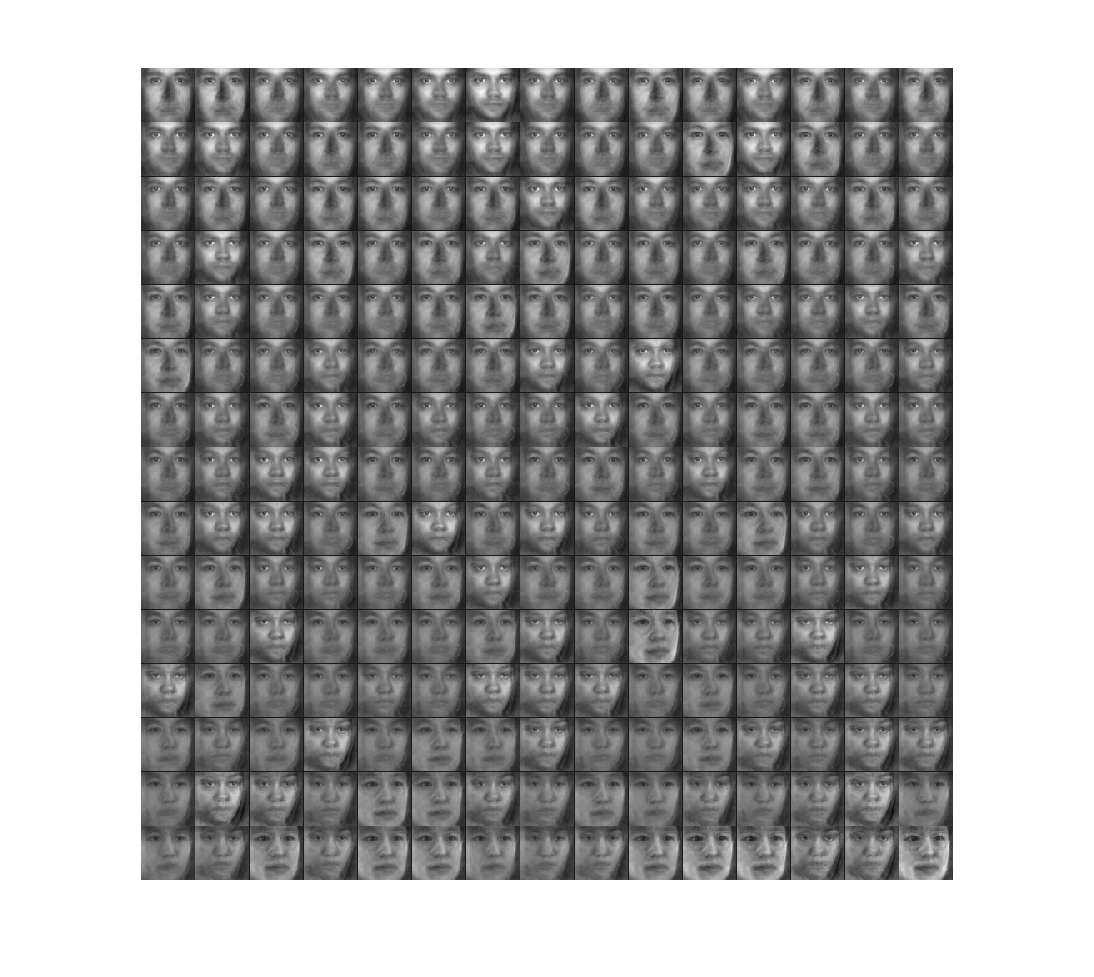
\includegraphics[width=\textwidth]{images/faceNWblock1.eps}
    \vspace{-2\baselineskip}
    \caption{Block 1 (2 hidden unit)}
    \end{subfigure}
	\begin{subfigure}[b]{0.5\textwidth}
    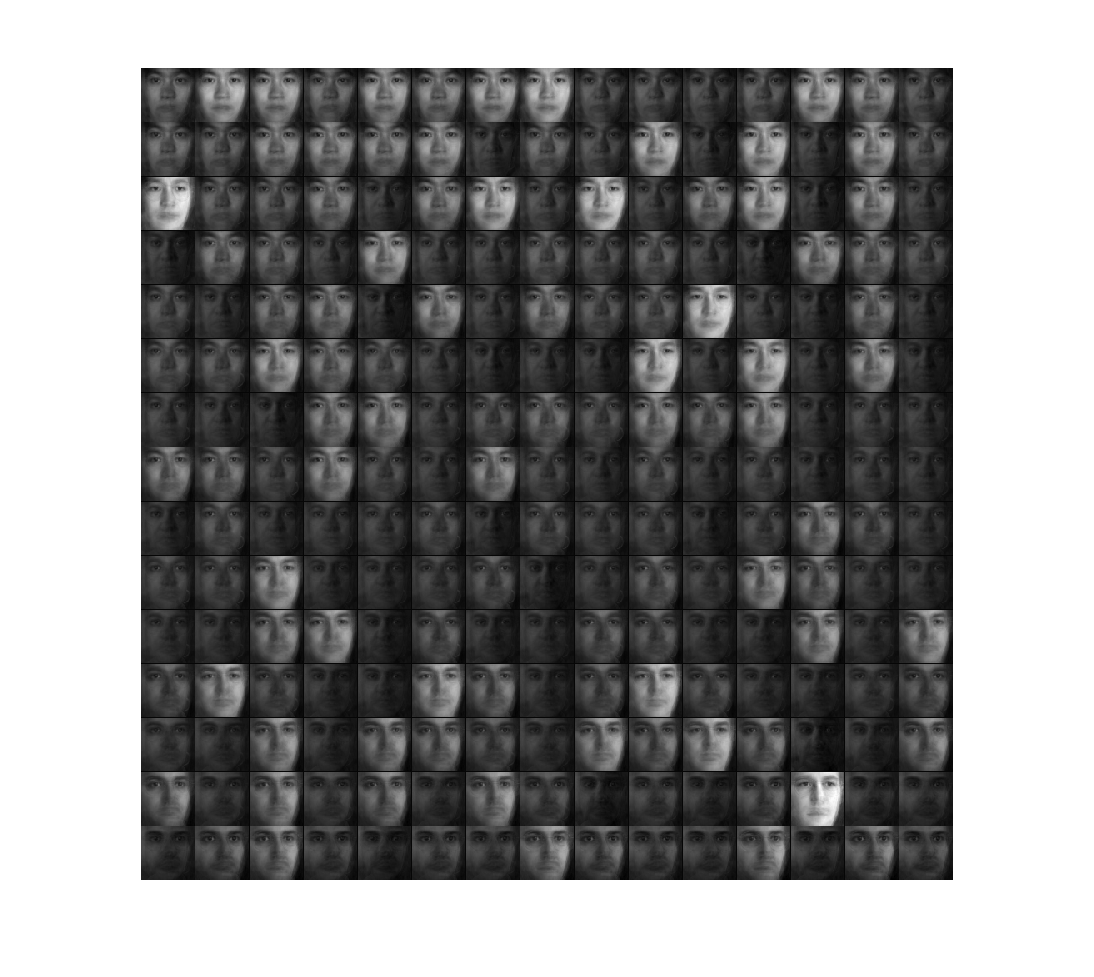
\includegraphics[width=\textwidth]{images/faceNWblock2.eps}
    \vspace{-2\baselineskip}
    \caption{Block 2 (2 hidden units)}
    \end{subfigure}
    \begin{subfigure}[b]{0.5\textwidth}
    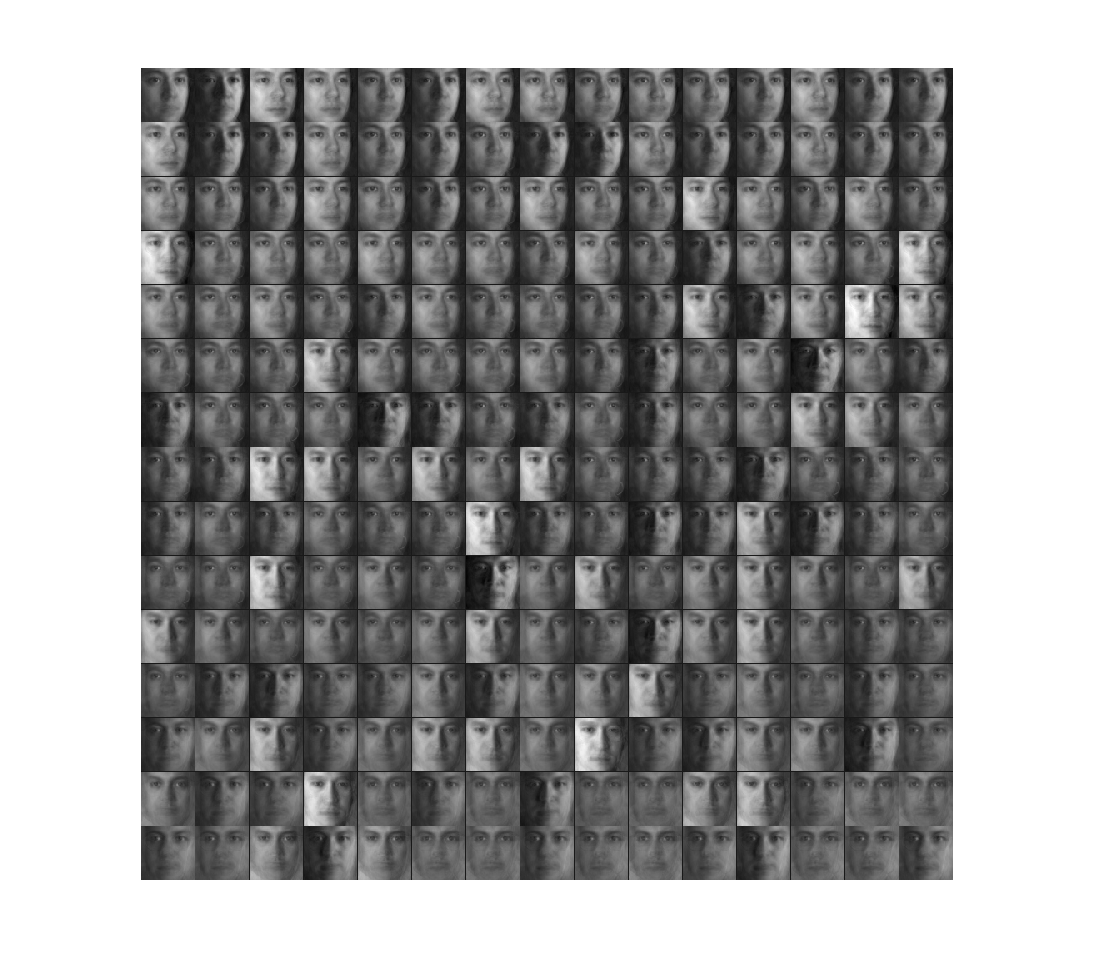
\includegraphics[width=\textwidth]{images/faceNWblock3.eps}
    \vspace{-2\baselineskip}
    \caption{Block 3 (2 hidden unit)}
    \end{subfigure}
    \caption{Generated face samples from \textbf{model C}. Block 1 means that we sample for block 1 and fixed others (with mean), and etc.}\label{fig:animals}
    \label{fig:FacesamplesModel3}
\end{figure}



\begin{figure}
\centering
    \begin{subfigure}[b]{0.5\textwidth}
    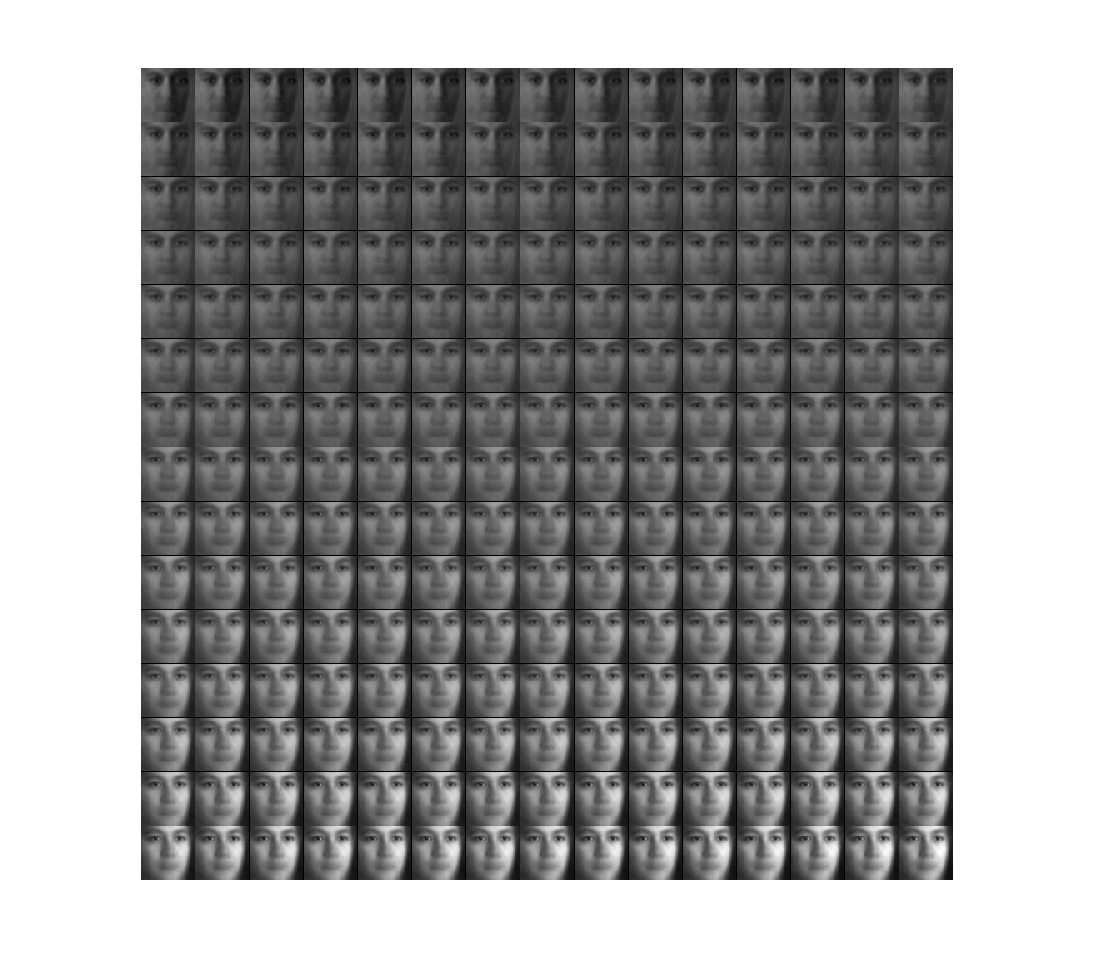
\includegraphics[width=\textwidth]{images/faceBlock1.eps}
    \vspace{-2\baselineskip}
    \caption{Block 1 (1 hidden unit)}
    \end{subfigure}
	\begin{subfigure}[b]{0.5\textwidth}
    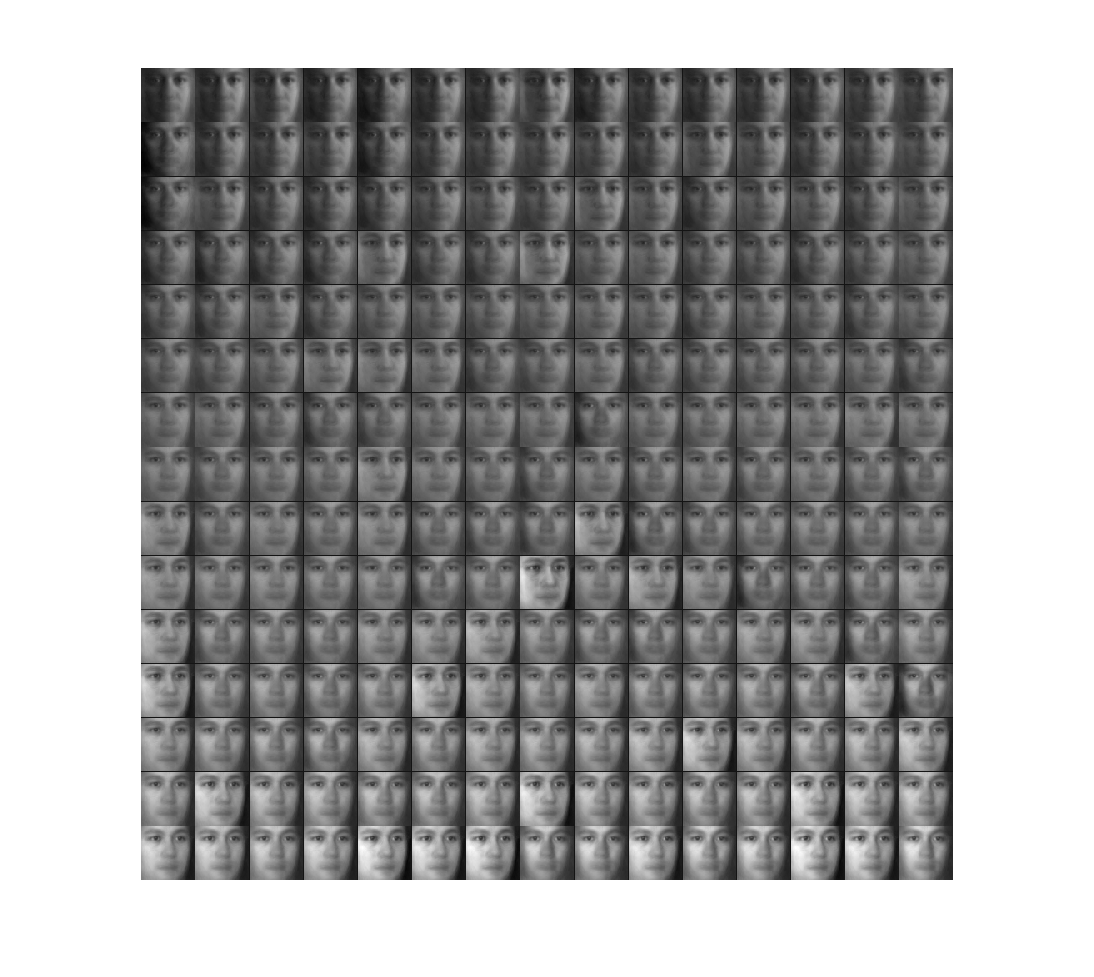
\includegraphics[width=\textwidth]{images/faceBlock2.eps}
    \vspace{-2\baselineskip}
    \caption{Block 2 (4 hidden units)}
    \end{subfigure}
    \begin{subfigure}[b]{0.5\textwidth}
    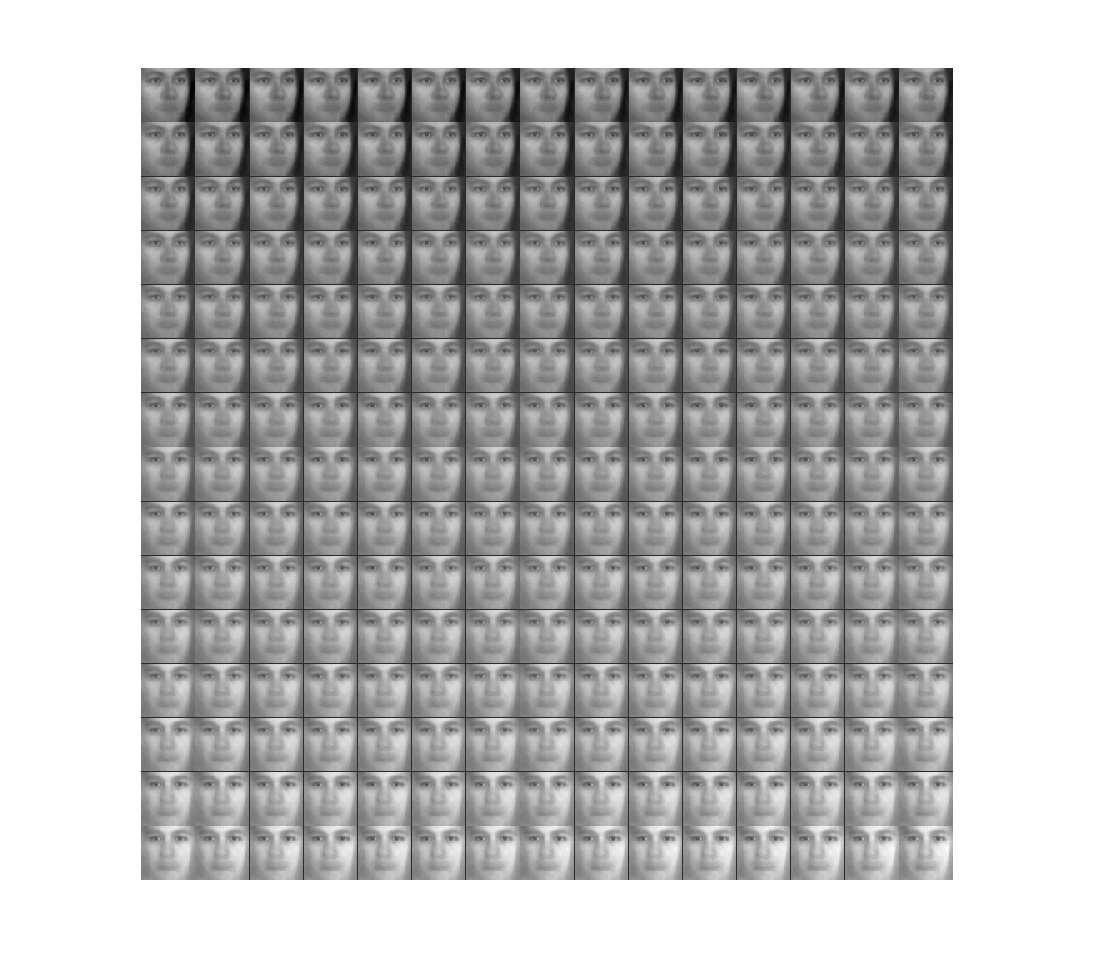
\includegraphics[width=\textwidth]{images/faceBlock3.eps}
    \vspace{-2\baselineskip}
    \caption{Block 3 (1 hidden unit)}
    \end{subfigure}
    \caption{Generated face samples from \textbf{model D}. Block 1 means that we sample for block 1 and fixed others (with mean), and so on}\label{fig:animals}
    \label{fig:Facesamples}
\end{figure}


\begin{figure}
\centering
    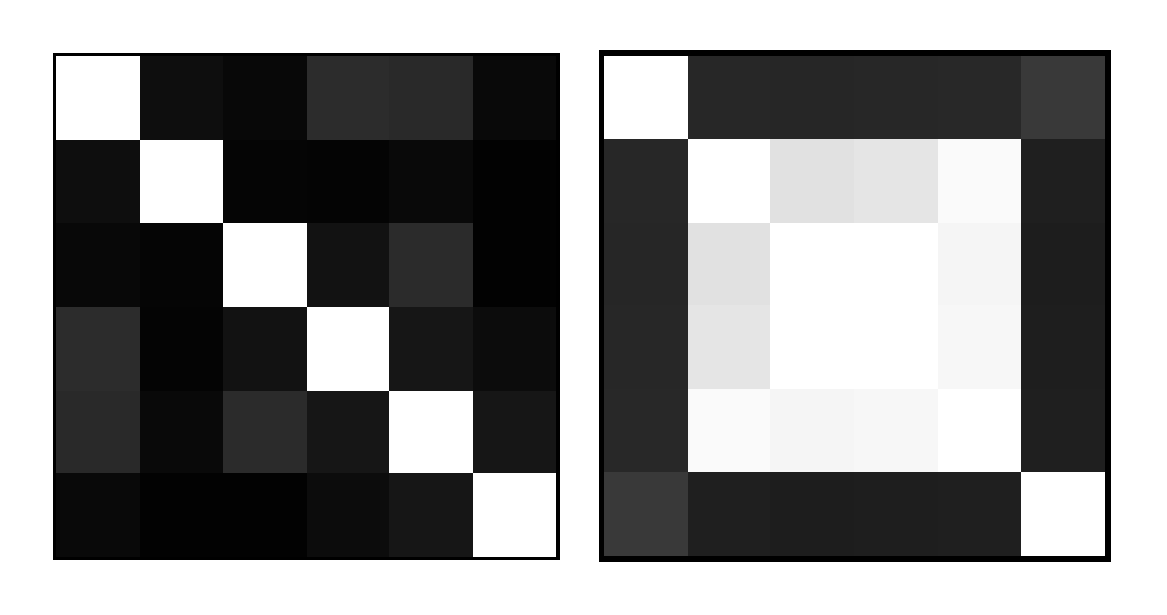
\includegraphics[width=0.8\textwidth]{images/faceCorrCompare.eps}
    \caption{Correlation matrix from learned representations. The left figure is for model C, and the right figure is for model D}
    \label{fig:FacesamplesModel3}
\end{figure}






\subsection{Norb dataset}

\begin{figure}
\centering
    \begin{subfigure}[b]{0.5\textwidth}
    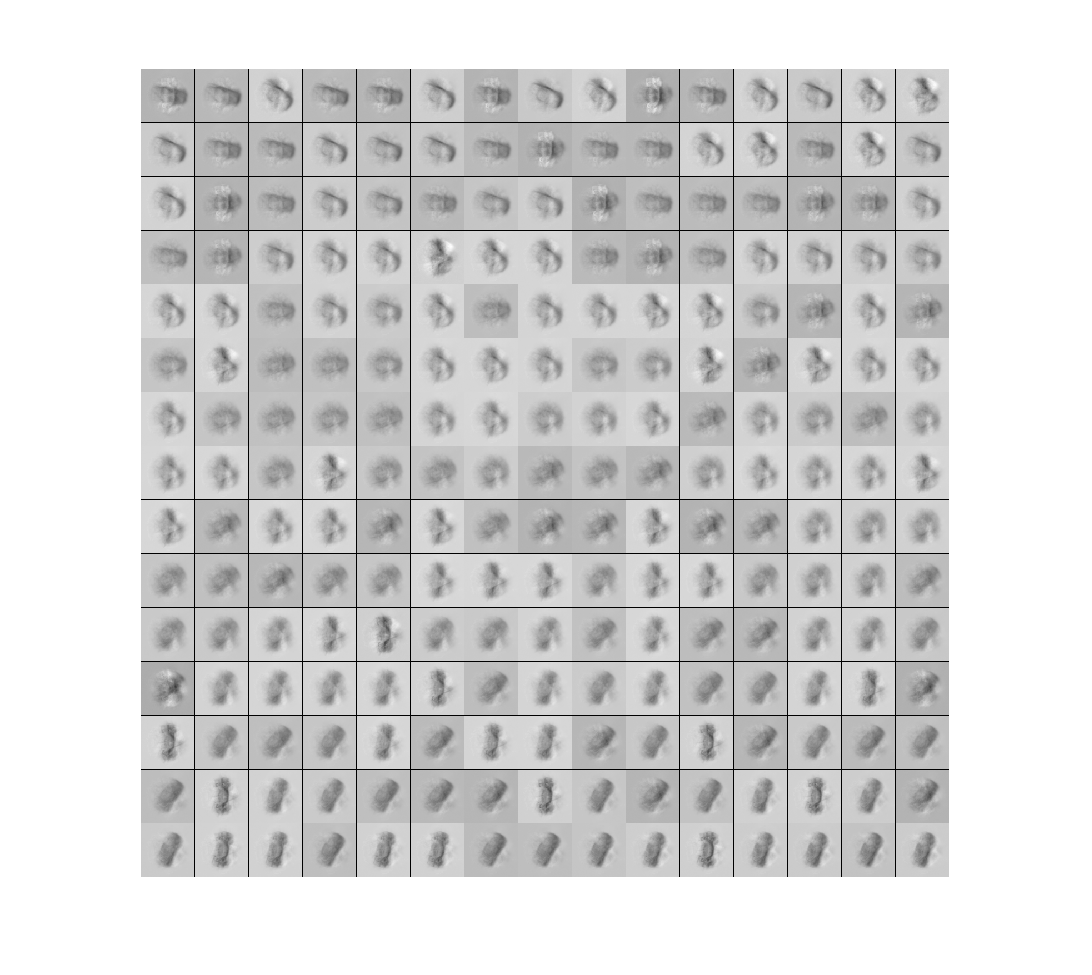
\includegraphics[width=\textwidth]{images/norbNWblock1sample.eps}
    \vspace{-2\baselineskip}
    \caption{Block 1 (2 hidden unit)}
    \end{subfigure}
	\begin{subfigure}[b]{0.5\textwidth}
    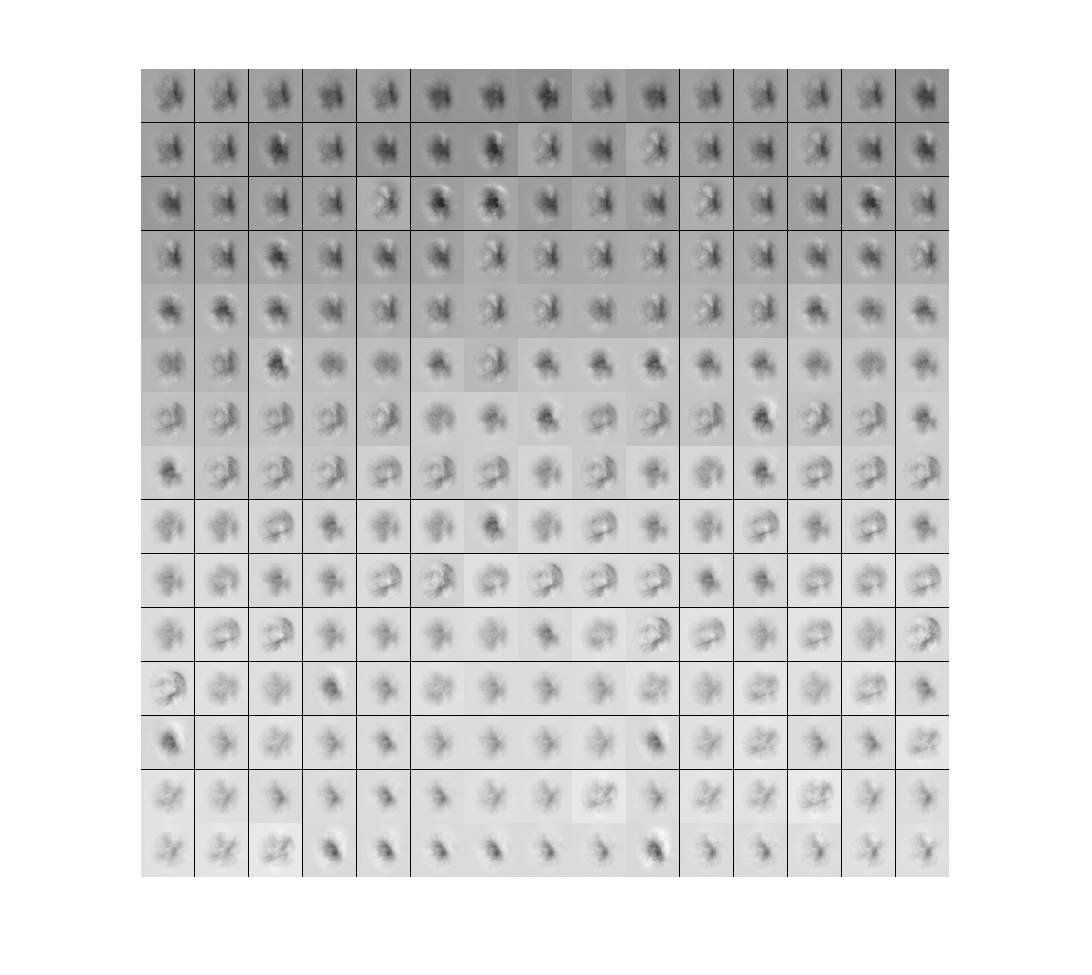
\includegraphics[width=\textwidth]{images/norbNWblock2sample.eps}
    \vspace{-2\baselineskip}
    \caption{Block 2 (2 hidden units)}
    \end{subfigure}
    \begin{subfigure}[b]{0.5\textwidth}
    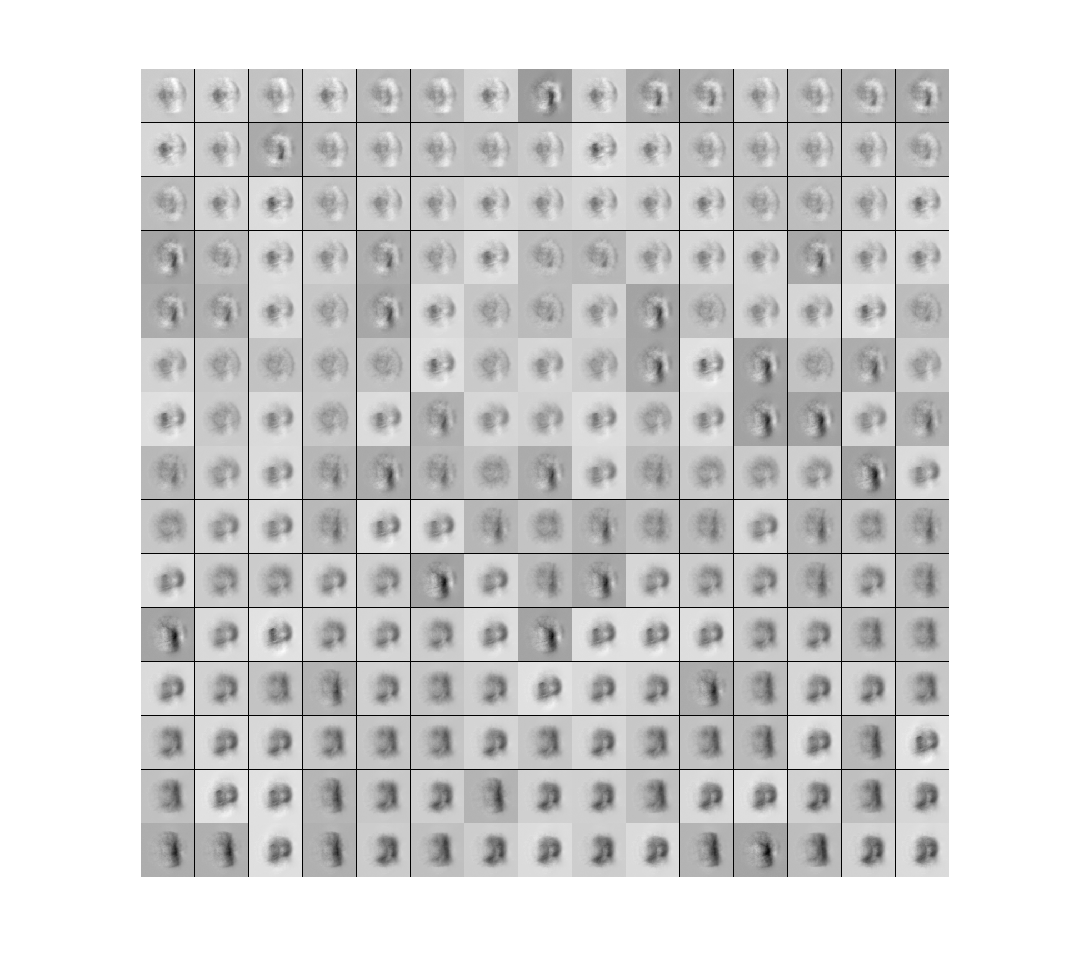
\includegraphics[width=\textwidth]{images/norbNWblock3sample.eps}
    \vspace{-2\baselineskip}
    \caption{Block 3 (2 hidden unit)}
    \end{subfigure}
    \caption{Generated face samples from \textbf{model C}. Block 1 means that we sample for block 1 and fixed others (with mean), and so on.}\label{fig:animals}
    \label{fig:norbsamples}
\end{figure}

In order to better understand the performance of our models. We also evaluate them on more complex datasets, which has three factors of variation. We use $6$ hidden units and we set the number of blocks to $3$. The Figure~\ref{fig:norbsamples} shows the generated samples from Model C. We can easily see that the block 1 encodes orientation, block 2 encodes the brightness and block 3 encodes the identity.



\section{Discussion and Future Work}
In this paper, we propose a generative model for learning disentangled latent representations. From the preliminary results, we could easily see that the learned representations have the effects of disentangling, although it's hard to get the complete disentangled representations from our methods. But this is reasonable since we haven't use any other information such as labels.  

\textcolor{blue}{other discussion points}

For the future work, we plan to extend our current model to nonparametric by using Dirichlet process, which should be straightforward.  

\section{Conclusion}
In this paper, we present new probabilistic models for learning the disentangled representations. We first provide the methods for the problem with known block structure, and later we generalize it to the case of unknown block structure by putting variable clustering prior. For the future work, we plan to extend it to the nonparametric case when the number of blocks is also unknown. More empirical evaluation can be conducted on more complicated datasets.  


\begin{figure}[h]
\begin{center}
%\framebox[4.0in]{$\;$}
\fbox{\rule[-.5cm]{0cm}{4cm} \rule[-.5cm]{4cm}{0cm}}
\end{center}
\caption{Sample figure caption.}
\end{figure}


\bibliographystyle{apalike}
\bibliography{ref}

\end{document}
